\documentclass[preprint]{elsarticle}
\usepackage[latin1]{inputenc}
\usepackage[english]{babel}
%\usepackage[T1]{fontenc}
%\usepackage{textcomp}
\usepackage{graphicx}
\usepackage{color}
%\usepackage{setspace}
\usepackage{url}

\begin{document}

\begin{frontmatter}

%%%%%%%%%%%%%%%%%%%%%%%%%%%%%%%   TITLE   %%%%%%%%%%%%%%%%%%%%%%%%%%%%%%%

\title{Studying Real Traffic and Mobility Scenarios for a Smart City Using a New Monitoring and Tracking System}
% Antonio - A ver qué os parece el título. ;D

%%%%%%%%%%%%%%%%%%%%%%%%%%%%%%%   AUTHORS   %%%%%%%%%%%%%%%%%%%%%%%%%%%%%%%

\author{A.J. Fernández-Ares$^1$, A.M. Mora$^1$, M.G. Arenas$^1$, P. García-Sanchez$^1$, G. Romero$^1$, V. Rivas$^2$, P.A. Castillo$^1$, J.J. Merelo$^1$}
\ead{\{antares, amorag, mgarenas, pablogarcia, gustavo, pacv, jmerelo\}@ugr.es, vrivas@ujaes.es}
\address{$^1$ Departamento de Arquitectura y Tecnología de Computadores.\\ ETSIIT - CITIC. University of Granada, Spain\\
$^2$ Departamento de Informática. EPS. Universidad de Jaén, Spain}

%\maketitle

% Si quieres que el resumen (y el paper) cumpla lo prometido por el
% título 1. Debes decir cuáles con los "temas reales" de una smart
% city.
% 2. Debes examinar el estado del arte en esos problemas. ¿Cómo se
% resuelven? 
% 3. Debes presentar la solución y en qué mejora el estado del
% arte. ¿Precio? ¿Disponibilidad? ¿Problemas que realmente resuelve? 
% 4. Presentar _solo_ lo que se refiera a smart cities. Pista: las
% discotecas no tienen nada que ver.  - JJ

% Antonio - ya está mejor definido el título.
% Esto es una prueba de concepto de MOBYWIT, no pretendemos mejorar el estado del arte en cada problema, los cuales ya han sido profundamente estudiados por otros autores, sino mejorar el estado del arte en los dispositivos que hay de detección y monitorización de tráfico y personas, ofreciendo una solución que sirve en varios escenarios diferentes y favorece la obtención de información útil en cada uno de ellos, para solucionar problemas de la ciudad que ayudarían a que ésta fuese una Smart City.
% Lo explicaré mejor a lo largo del paper.
% Además, el estado del arte tengo que completarlo con esa parte.
% Respecto a la disco, se puede considerar parte de una Smart City por dos cosas: por marketing y siendo un 'Smart Building', que pueda optimizarse energéticamente y en cuestiones de seguridad.
% Lo aclararé también.

%
%%%%%%%%%%%%%%%%%%%%%%%%%%%%%%%%%   ABSTRACT   %%%%%%%%%%%%%%%%%%%%%%%%%%%%%%%%%
%
\begin{abstract}
This paper presents a novel mobility monitoring system and some of its applications to address problems that would be solved in a Smart City, such as the optimization of traffic flows in terms of trip-time and security (Smart Traffic), and the improvement of security or energetic issues inside buildings.
The system tracks the movement of people and vehicles monitoring the
radioelectric space, catching the  WiFi and Bluetooth signals emitted by personal(smartphones) or on-board (hands-free) devices. 
A study has been conducted in four different real scenarios,
i.e. with real data gathered by the system: two related with people's
mobility (a public building and a discotheque); and two focused in
traffic tracking (urban and intercity roads). 
The analysis has consisted on the application of different data mining techniques to extract useful knowledge, traffic forecasting methods to perform accurate predictions, and statistical analyses to model and validate the system
reliability (using other real data sources).
The obtained results show the viability and utility of the system in all the cases, along with some of its multiple applications for solving different issues in a city. 
% Antonio - Solucionados los comentarios
\end{abstract}

%
%%%%%%%%%%%%%%%%%%%%%%%%%%%%%%%%%   KEYWORDS   %%%%%%%%%%%%%%%%%%%%%%%%%%%%%%%%%
%
\begin{keyword}
Smart traffic \sep Transit indicators \sep Traffic forecast \sep Mobility analysis \sep Smart City \sep Internet of Things
\end{keyword}

\end{frontmatter}


%-------------------------------------------------------------------------------
%%%%%%%%%%%%%%%%%%%%%%%%%%%%%%%   INTRODUCTION   %%%%%%%%%%%%%%%%%%%%%%%%%%%%%%%
%-------------------------------------------------------------------------------

\section{Introduction}
\label{sec:intro}

Nowadays, the transformation of any city into a Smart City, with better performance (saving energy, citizen's time, resources, costs), is a process that must be supported by powerful and reliable technologies, methods and systems. 
To this aim, a mobility monitoring system is one of the most useful, since the data which provides can be used to enhance several services in the city, or in specific buildings inside it.

The most common systems gather traffic information (mainly vehicles pass-by) using several kind of devices, such as pneumatic tubes, loop detectors, floating vehicles or automatic Optical Character Recognition (OCR) \cite{rodrigue2013geography}. However most of these systems are not able to identify and follow the same vehicle along the road network. 
% ¿OCR no? - JJ
% Antonio - Sí, por eso pone most of them.
Those that can do it are very expensive so they are just placed in very specific points of the roads.

The local, regional or national governments use these data aiming for improvements in the maintenance of roads and services, computing a road deterioration factor based on the affluence of vehicles, for instance. In addition, useful traffic statistics can be obtained, which would help to forecast traffic jams, for example.
This information can be directly used inside a city in several ways, from improving the traffic flow (adjusting the synchronisation of traffic lights or defining the best traffic sense on every street), to the end-users (drivers), who can profit by optimally planning their trips according to the current, or future, status of the traffic flow. 
That's the reason why traffic information must be reliable. 

This paper presents a monitoring system able to collect people's and vehicles mobility data, and also able to track them by means of a grid of devices (nodes) connected to a central server. This allows the easy construction of traffic flow models or mobility graphs. The proposed system is formed by low-cost devices (around 100\$ each one), which is another advantage over the usual monitoring systems, because the cost is an important factor for authorities which
tend to install the simplest and cheapest monitors. 

The device, a highly improved version of the one presented in
\cite{castillo2014_book_sipesca}, is based in a single-board computer
which monitors the radioelectric space capturing Bluetooth (BT) and
WiFi signals emitted by other devices,  mainly
smartphones or hands-free systems on vehicles, which are detected and
identified by means of their Media Access Control number (MAC) - which
is unique - and stored as a traffic `event' (pass-by). 
% Antonio - ¿Se os ocurre un nombre mejor para los 'pasos'?
% step desde luego que no. pass-by en todo caso - JJ
% Antonio - me quedo con 'event'
Thus, depending on the position of the monitoring device (node), we could
gather information about specific people's or vehicles'
displacements. In order to respect the person's privacy as well as
data protection laws, the MAC is encrypted using a one-direction
process before storing it, so, we cannot associate a captured MAC with
any person. 
% habría que asegurar, además, que ese proceso de cifrado no se puede
% replicar. ¿Qué clave usa? - JJ
% Antonio - No se puede replicar, pero que lo aclare Antares.
% Antares: Se parte de los 48bits de la MAC a 160 bits de SHA-1, por lo que el riesgo de colisión es imposible. Pero, no creo que sea relevante.

To prove the reliability and utility of this system are also objectives of this work, so, four different real scenarios are presented and the collected data analysed in order to demonstrate its value for solving different problems in a city. These scenarios are focused in the city of Granada (Spain), in which real traffic/mobility data have been gathered. They are namely: a discotheque, a public building of the University, a highway between Granada and Málaga; and one of the main streets in the city.  
% yo dejaría la facu y la discoteca. Son totalmente diferentes. Salvo que quieras contarlos por temas de carga o lo que sea, no tienen nada que ver. 
% Antonio - son estudios sobre movilidad de personas. Si se consiguen mejorar cuestiones de seguridad, por ejemplo, yo los considero parte de una Smart City.
Several devices or nodes have been deployed in each scenario.
The huge amount of data produced have been processed using \textit{Big Data} 
% Antonio - Meto también lo de Big Data que es otra 'palabra clave'
% del Special Issue. ;D. Antares, esto es Big Data, ¿no? :D 
% No es big data. Es mucho data. Y "deeply processed" no sé qué
% significa - JJ
techniques, transforming or summarizing them, in order to conduct
further analyses. Different methods have been applied, such as Data
Mining, Time Series Forecasting, In/Out (Origin/Destination) matrices,
or statistical procedures. % pero ¿con qué objetivo? - JJ
The aim was to extract useful information and reach clear conclusions
which can lead to enhance the performance of different aspects in every scenario, proving the value of this monitoring system as a
tool to improve different issues inside the city and buildings. Thus,
the system would be suitable to be part of a \textit{Smart City}. 

% Antonio - Hay que hacer referencias a Smart City a lo largo del paper. ;)

The use of these devices can be framed in the paradigm of Internet of
Things (IoT), as we are integrating communications and technologies
for identification and tracking, with the use of wireless sensors and
actuator networks \cite{Atzori2010IoTSurvey}. 

The rest of the work is structured as follows. Section \ref{sec:soa}
presents the background and state of the art on the main topics of the
work: traffic and mobility monitoring, traffic series forecast, and
smart city tools, among others. 
Then, our monitoring device is introduced in Section \ref{sec:mobywit}.
After this, there are four sections devoted to describe and analyze the different scenarios, namely: Section \ref{sec:disco} explains the discotheque scenario and the methods applied to its data, Section \ref{sec:etsiit} presents the study on the University building, Section \ref{sec:traffic} shows the analysis on the highway traffic, and Section \ref{sec:city} comments the scenario on the street of Granada.
Finally, Section \ref{sec:conclusions} plots the conclusions that we
have reached in the work. 


%----------------------------------------------------------------------------
%%%%%%%%%%%%%%%%%%%%%%%%%%%%%   STATE OF THE ART  %%%%%%%%%%%%%%%%%%%%%%%%%%%
%----------------------------------------------------------------------------


\section{Background and state of the art}
\label{sec:soa}

Several technologies are used to collect data and gather information about the 
state of the roads. Traffic monitoring technologies can be classified as 
\textit{intrusive}, installed in the pavement, and
\textit{non-intrusive}, without contact with the road, causing minimal
effect on the traffic flow \cite{martin2003detector}. 

As stated in previous section,the main technologies currently used include pneumatic tubes, inductive loop detectors and automatic recognition systems (or OCR), among others \cite{rodrigue2013geography}.

Pneumatic tubes are placed on top of the lane to detect vehicles by the change 
in pressure generated when a vehicle passes over the tube. 
An inductive loop detector is a wire embedded into the roadway usually
in a square configuration. An electric current is sent to the wire and
when a metal surface with certain minimum area pass or is stopped
above a pulse is triggered and detected. The main drawback of these
two systems is that they are unable to identify the vehicle detected
by the sensor. This way, the highly desired origin/destination
matrices cannot be obtained. Just the number of vehicles and their
type can be guessed. This count, although valuable, does not allow us
to know many traffic flow characteristics like, for example,
repetitive passes of the same vehicle. Because of their relatively
high cost of installation and maintenance it is not feasible to
install them all over our roads. That is why we can only see them on
major roads, cities and points of special interest. 

Finally, the automatic recognition technology has experienced an increase in 
recent years due to its ability to detect individual vehicles without relying 
on in-vehicle systems. Video image detection is a good example; in this case a 
trip line and/or tracking is used to record traffic data. Furthermore, they 
are used for automatic detection of incidents on the road. That is the main 
advantage over previous information systems. However, system reliability might 
not be the best, as weather may limit accuracy. Moreover, these systems are 
very expensive compared to the previously described \cite{skszek2001state}. 
Another problem has arisen recently with privacy. The Spanish Data Protection 
Agency (Agencia de Protección de Datos) considers the car license plate number 
as personal data. Thus, user consent is required for it to be saved.

There are many different companies working in the traffic information
field. Some of the more relevant are: 

\begin{itemize}
\item Bit Carrier \cite{mendez2011system,BitCarrier}: It offers a traffic 
management system based in BT to count people and commercial routes 
(pathsolver). Its technology was deployed in highways managed by Abertis for 
traffic flow control and monitoring. Actually it has a network of 150 devices 
in Catalonia (Spain) capable of tracking 200000 people every day.
\item Trafficnow \cite{Trafficnow}: Offers a traffic flow control centre for 
small towns. It requires a net of BT sensors. %A pilot experience has been deployed in Vigo.
\item Traffax Inc \cite{TraffaxInc}: It is a company that has also used 
BT for calculating origin/destination and transport time matrices.
\item Savari Networks \cite{SavariNetworks}: It offers the commercial 
product StreetWAVE for real-time traffic monitoring.
\item TrafficCast \cite{TrafficCast}: They have developed predictive models 
in different cities based on different technologies, such as video cameras, BT devices, and RFID tags included in the vehicles wanted to be followed.
\end{itemize}

% Antonio - Maribel, voy a recortar cosillas, que te enrollas incluso más que yo. No te enfades, porfa. XD
Traffic has been extremely exploited as a research field, mainly focused on the forecast of future flows considering the current information as a Time Series.
The forecasting of these flows in any transport system plays an important role for either alleviating urban congestion, or for adjust traffic control and guidance systems. The aim is to create an intelligent transportation system (ITS) which strongly depends on the capability to predict traffic conditions at least in the short-term (less than one hour into the future), since medium- and long-term predictions are barely accurate and reliable. These are nowadays a hard problem to solve in general Time Series \cite{ParrasGutierrez2014433}.
% Antonio - supongo que el medio y largo plazo no es que ayude, sería estupendo, sino que es muy difícil que sea preciso. ;)
% Antonio - quito la segunda referencia, ya que va de otras cosas y seguramente nos van a dar un toque por la extensión del artículo. :D
With a short-term forecasting the traffic control systems could be self-adapted continuously. For example, a traffic light could adjust its red or green time depending on the short-time forecasting of the closer streets. 

%Medium-term or long-term could to be useful if there are special conditions in a medium or long time period although nowadays the results of this research are not outstanding and it is an open question for many research groups, but usually in other subjects like time series in general \cite{ParrasGutierrez2014433} or economic development and political decisions \cite{longTermBussines2014}.


There are many works related with traffic flow forecasting, each of them approaching the problem with different models \cite{SurveyKumar2007} such as Kalman Filter Theory \cite{ASJC:ASJC1051}, Markov Chain models \cite{Qi201495}, non-parametric methods \cite{Noparametrico2014}, simulation models \cite{simulaciontrafico2012} or ``Big Data'' based approaches \cite{SurveyKumar2007}.  %(buscar referencias recientes de cada una y ponerlas si queremos ampliar este párrafo)
% Antonio - pos eso. ;D
%

Being the traffic flow forecasting a trending topic several surveys can be found, such as \cite{Survey2004} and \cite{SurveyKumar2007} but the best is \cite{SurveyBolshinsky2012}, since Bolshinsky and Friedman complete the information that the previous ones just compile, and give an added value to their work including the used techniques, the input data for each contribution, and the used hardware architecture, whenever the original paper described it. There are also specific surveys for one of the traffic flow forecasting types, like \cite{Vlahogianni2014} where the focus was not the approaches nor the results of the reviewed papers, but the focus or goals and the scope where each paper could be classified, for example if the work is focused on forecasting or presents the collecting data system as main contribution.



During the last years, the researches even assimilate new technologies
for data analysis like ``Big Data'' \cite{TrafficFlowPredictionWithBigData2015} or Cloud-Computing
approaches \citep{CloudComputing2014}. In the first one, Yisheng
et. al. face the traffic flow forecasting problem using temporal and
spatial models at the same time, using simple forecasting models and
assembling them in a global complex system. The results provide a time
and a spatial place for each prediction. The second work, by Zhaosheng
Yang et al., presents a traffic flow prediction model for large-scale
road network using Cloud-Computing techniques. Thus, it implements
successfully a Genetic Algorithm (GA) for optimizing a Support Vector
Machine (SVM) getting a higher prediction accuracy and a smaller
running time.  



Several recent publications present spacial issues related with the
scope, such as \cite{Zhang20141}, which includes the latest advances in
traffic forecasting research having in mind the time and the space variables.  
% Antonio - ¿como cuáles?
Other works propose conducting forecast traffic flows and trip times
\citep{Dong201420}, \cite{Zou201433} using spatial-temporal patterns
of the congested and non-congested traffic. Also papers with new
real-time forecasting approaches \cite{Zhang201465} or improved and
renewed proposals such as \cite{Wang201479}, which improves the
Bayesian combination method (BCM) proposed by Petridis et al. in 2001,
or \cite{Qi201495} which improves freeways short-term prediction using
a Markov Model. 


In the present work, a study on traffic forecasting is conducted (in Section \ref{sec:traffic}), however it applies classical methods, because the aim is to show the value of the data gathered by our system in the comparison with the data collected by the Spanish Traffic Agency using an inductive loop detector, which is also studied.
Thus, our contribution on this line is the use of real traffic Time Series, created from the data extracted from our traffic `events' (WiFi and BT detections).

% Antonio - he movido este texto que es más de background a esta sección. ;)
Another line of study in our paper is the personal tracking or people's mobility. It is studied for many reasons, several of them involving profit: conversion rate, marketing effectiveness or staff planning are some of the best known \cite{stanton1967fundamentals}. Conversion rate is the percentage of visitors who effectively make a purchase. It can show you if a shop improvement (or decline) is due to more people visit it, or more of the visitors finally buy something. Shopping mall professionals study people's behaviour in order to know if their marketing techniques are paying off. In the same line, stuff planning is directly related with the amount of visitors, as well as the maintenance and cleaning needs.

Other reasons are more practical than commercial: How many people visit a public building? When? It will help to improve the planning of the provided services, heating or cooling of the building, facility cleaning, staff shifts and so on. In a museum or a sport stadium you can adjust many parameters to help people enjoy from a better experience while raising the profits.

The technology for counting/tracking people has evolved over time. At the beginning infrared beam counters \cite{Hashimoto199850} were used. These were cheap but prone to failures, like when two persons pass a door together. Thermal counters \cite{635472} were used next. Also cheap but with serious limitations like the short distance from the counting device to the people being counted. Latest technology use video cameras \cite{4107051,Schofield19961421} and WiFi \cite{7134066,7130402}, or Bluetooth \cite{6526732,nicolai2007relationship} detectors. 
% Antonio - esto es importante, habría que extenderlo y compararlo con lo nuestro, ya que se podría parecer. Aparte de la cita. ;D
Video devices are more expensive as is the software in charge of image processing, more expensive in terms of resource consumption. On the positive side, now we can do many more things than counting people. We can track their paths and behavior. Radio signal is also a great method to track people, as powerful as video but cheaper in terms of hardware price and algorithmic cost. Moreover, the range of detection is wider, 100m approximately.

Our approach is based on WiFi and BT \cite{824570} detection, but focused on people's personal devices from which an unique identifier can be extracted and, after anonymisation, stored. This makes it easy to track these people on a building for instance, just deploying a fair number of monitoring devices. With the advantage of a cheaper price than other systems, such as video ones, and also the possibility of creating origin-destination flow matrices or any other desired movement model.

The idea of using BT personal devices is not new an has been tested by many previous researchers. In \cite{nicolai2007relationship} Tom Nicolai, like us, used statically placed BT detector to track people. Also in this work from Morrison \cite{morrison2009visualisation} the same procedure is followed to follow spectators activity on a stadium. Kostakos used this same idea to follow people trips in public transportation buses \cite{kostakos2008using}.
A good starting point to learn about the issue is \cite{6526732} with the additional originality of mixing stationary detectors with dynamic ones to estimate crowd density in a soccer stadium during a championship.

Also the idea of tracking people with their personal WiFi devices is not new. As more and more people use it every day it is becoming one of the best method to follow them. This idea has been put to practice recently by several authors. Wei Xi in \cite{6847958} demonstrates how this method can count people with great accuracy. Gabe Fierro in \cite{Fierro:2012:ZOC:2422531.2422572} use it to measure the occupancy level of a building without requiring additional infrastructure.

By joining BT and WiFi we pursue to increase the detection rate further than most people has achieved. Apparently it can seem redundant but the detection likelihood is higher. We need to study more deeply the improvement of the combined detection but on average we detect a 80\% of WiFi devices and a 20\% of BT. BT is specially important for the detection of cars because it is technology include in almost every new car. The same is true for WiFi and smartphones. Even when people disconnect WiFi devices keep on sending signals.

% TODO: ANTONIO - Meter estado del arte en Smart City y enlazar con lo de movilidad.

*** COMPLETAR ***

%------------------------------------------------------------------------------
%%%%%%%%%%%%%%%%%%%%%%%%%%%%%%%%%%  MOBYWIT  %%%%%%%%%%%%%%%%%%%%%%%%%%%%%%%%%%
%------------------------------------------------------------------------------

\section{MOBYWIT}
\label{sec:mobywit}

% en estos dos párrafos modificaría un poco la redacción como os comenté  [pedro]
% Antonio - No tengo las propuestas...
This device was designed by one of the authors and it is based in a
single-board computer, Raspberri
Pi\footnote{https://es.wikipedia.org/wiki/Raspberry\_Pi}. It has two
USB cards, namely a Bluetooth (BT) and WiFi ones, and it uses their
interfaces in monitor mode, scanning the radioelectric space searching
for BT devices and beacon frames (for WiFi). 

Every device, called MOBYWIT (Mobility by Wireless Tracking) is formed
by a hardware and a software layer very interconnected. It is part in
the whole monitoring system, which also includes cloud-based storage
and computing services. The software architecture of the whole system
is shown in Figure \ref{fig:mobywit}. 

\begin{figure}[ht]
	\begin{center}
		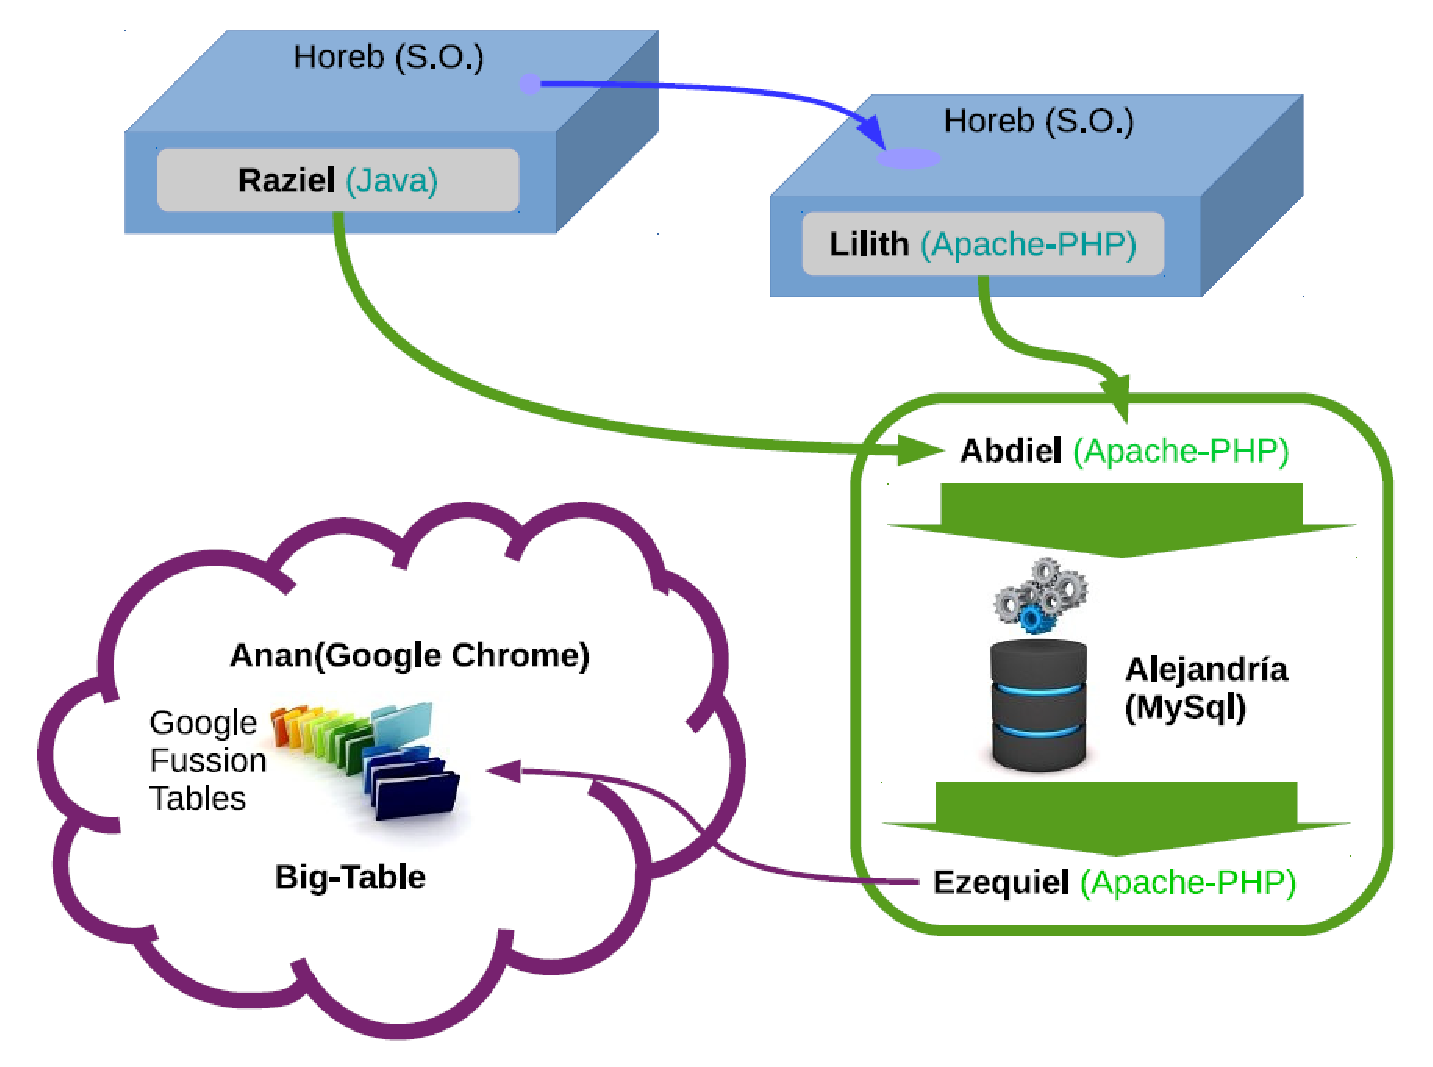
\includegraphics[scale=0.4]{imgs/mobywit.eps}
		\caption{MOBYWIT Monitoring system architecture}
	\label{fig:mobywit}
	\end{center}
\end{figure}

As it can be seen in that figure, there are six main parts in the software layer of the system, which are unidirectionally connected by a strict data flow. They are have been named as:
\begin{itemize}

\item \textit{Raziel}: This module is in charge of the detection of BT and WiFi devices as well as of their identification (extracting and encrypting the MAC) and the periodic submission of this information to the server. It is run in the device and implemented in Java.

\item \textit{Lilith}: This module acts as a gateway between the network of devices and the server. It allows the communications between nodes and between them and external networks. This component is also run in every device and implemented in PHP.

\item \textit{Abdiel}: This component implements a set of services for accessing the devices from `outside' (mainly for activate/deactivate or update them). In addition it performs the storage of gathered data (in blocks) in the server database. It is also implemented in PHP.

\item \textit{Alejandría}: This is the database of the system. It is a MySQL instance placed in a local server. It is optimized (using indexes and table partitioning) to provide a close to real-time processing and data service.
Ezequiel: This module is responsible of the publication of data in a cloud-based storage. It includes data mining, machine learning and forecast techniques to process these data in order to publish interesting or useful information about them.

\item \textit{Anan}: This is the cloud-based storage and services. It is based in Google technology so Anan stores and manages the data in a NoSQL format, by means of Google Fusion Tables. It also offers advanced visualization methods to be more usable and attractive for the end-user of the system.

\end{itemize}

In addition, and as it is shown in Figure 1, the device runs an specific Operative System, called \textit{Horeb}, which is a modification of the original Raspbian 3.10.24, adapted by MOBYWIT system designer to be more robust (to power fails, for instance) and reliable.

*** CONTAR CÓMO FUNCIONA AL DETECTAR ***
% Antonio - TODO: ANTARES, revisa esto porfa. ;)
There are several configuration parameters in the system, which sets important parts of the functionality, such as the intensity threshold to collect a received WiFi signal, or time limits to consider a device as obsolete or out of the range of the device.

Every detected `pass-by' or mobility `event' is associated to a detection time, obtained by NTP (Network Time Protocol). These `events' are stored initially in the device's memory. After some time (also set in a parameter) the information is sent, in blocks, to the server, to avoid an overuse/saturation of the network.


%----------------------------------------------------------------------------
%%%%%%%%%%%%%%%%%%%%%%%%   PEOPLE'S MOBILITY IN A DISCO  %%%%%%%%%%%%%%%%%%%%
%----------------------------------------------------------------------------

\section{Analysing people's mobility in a discotheque}
\label{sec:disco}

% ¿Por qué analizamos la discoteca?
Before using the device in other type of environments, we were
interested in checking its possibilities in an environment where
change is very fast and it is a priory possible to detect a big amount
of devices. That is why we decided to test MOBYWIT in a disco, using
using five MOBYWIT devices, deployed one in every of the three main
rooms, each one devoted to a different type of music and one on the main
entrance and the outdoor terrace. This scenario is interesting because
it is assumed that 100\% of users have a smartphone, thus it would be
a priori possible to track every single present device. The
electromagnetic scenario is also quite {\em heavy}, which presented a
challenge for testing the device.

A total of 2200 different devices were detected in one of the busy
nights (from a Thursday at 8 pm to Friday at 8 am), distributed per
node as it is shown in Figure \ref{fig:disco_data}. 

\begin{figure}[ht]
	\begin{center}
		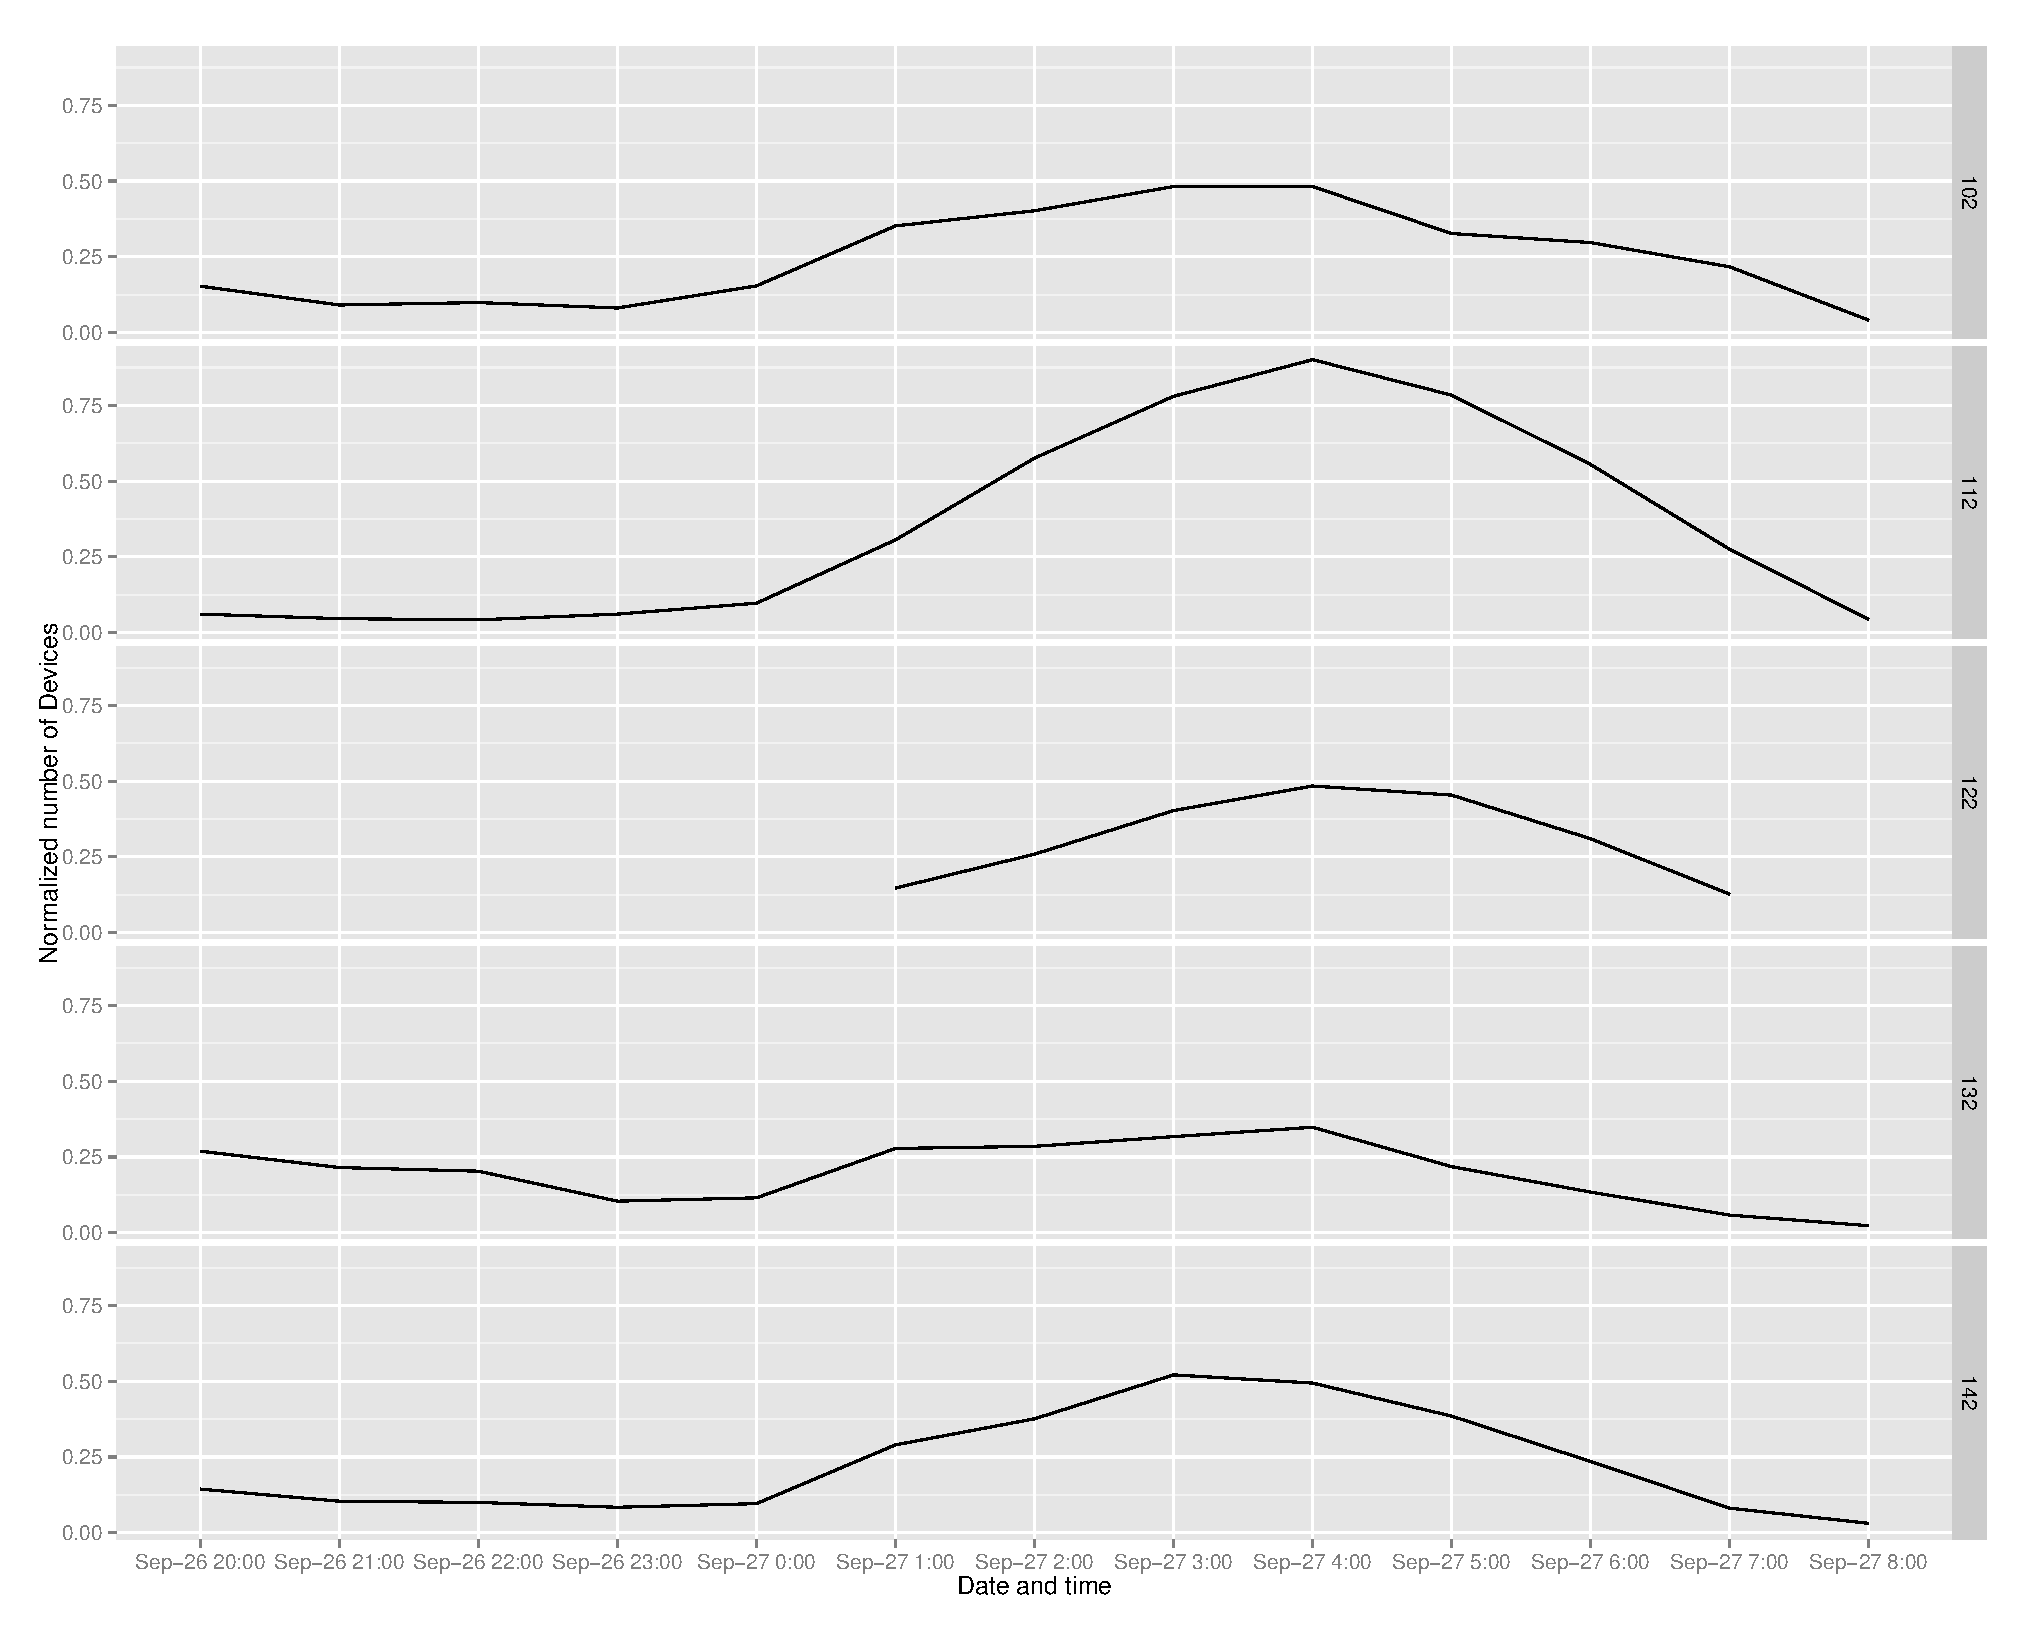
\includegraphics[width=\textwidth]{imgs/DISCO/time_series-linesPoints.eps}
		\caption{Detected devices in a night in the Discotheque scenario.}
		% Antonio - explicar lo que se ve en las gráficas (histograma y serie). Lo de la serie quizá no sea necesario
		\label{fig:disco_data}
	\end{center}
\end{figure}
% Antonio - Antares porfa, genera la gráfica correctas. ;)
% TODO: ANTARES - Gráfica correcta

These data have been processed and several variables have been
extracted from them, in order to apply clustering methods. % ¿Qué
                                % variables? ¿En qué estabas
                                % interesado? - JJ

% ¿Por qué haces clustering? 
The clustering study has been conducted by means of a Self-Organizing
Map (SOM) \cite{Kohonen90}, a feed-forward neural network
\cite{NN_Haykin94} that uses an unsupervised training algorithm and
nonlinear regression techniques to learn or find unknown relationships
among the set of variables that describe a problem. The main property
of the SOM is that it makes a nonlinear projection from a
high-dimensional data space on a regular, low-dimensional (usually 2D)
grid of neurons, called units. This grid can be later processed to
obtain the unified distance matrix (U-matrix) \cite{UmatUlts} which
uses SOM yielded neurons' codevectors (vectors of variables of the
problem) as data source, and generates a matrix where each component
is a distance measure between two adjacent neurons. Then, these
distances are codified as different colour shades in a graph. 
The U-Matrix graph allows visualise any multi-variable dataset in a two-dimensional display, which helps detecting topological relations among neurons and inferring about the input data structure in a straightforward visual manner. High values in the U-matrix represent a frontier region between clusters, and low values represent a high degree of similarities among neurons on that region, i.e. clusters. MATLAB 2009 along with SOM Toolbox \cite{SOMPAK} was used for the SOM analysis.

In order to analyse the data, several features have been extracted (generated) from the gathered `events', composing a pattern per device of its whole stay in the disco. These are described in Table \ref{tab:extracted_features_disco}.

\begin{table}[htpb]
\centering
{\scriptsize
\begin{tabular}{lll}
\hline\noalign{\smallskip}
Variable name & Description & Type\\
\noalign{\smallskip}\hline\noalign{\smallskip}
\texttt{entrance\_time} & First date/time when the device was detected & Date\\
\texttt{out\_time} & Last date/time when the device was detected  & Date\\
\texttt{stay\_time} & Number of seconds the device has been in the disco & Integer\\
\texttt{abs\_time\_node\_X} & Number of seconds the device has been detected\\
& in every node X (from 1 to 5) & Integer\\
\texttt{relat\_time\_node\_X} & Percentage of time the device has been detected\\
& in every node X (from 1 to 5) & Float\\
\texttt{relat\_night\_time\_node\_X} & Percentage of time the device has been detected\\
& in every node X (from 1 to 5) regarding the whole timetable\\
& of the disco & Float\\
%\texttt{non\_detected\_time} & Number of seconds the device has not been detected (but it still is in the disco) & Integer\\
\noalign{\smallskip}\hline
\end{tabular}
 \caption{Extracted features from gathered data in the discotheque. \label{tab:extracted_features_disco}}
}
\end{table}


The application of SOM + U-Matrix produces the graphs shown in Figure
%\ref{fig:som_disco_no_detec_0} and
\ref{fig:som_disco_sin_no_detec}.

%\begin{figure}[ht]
%	\begin{center}
%		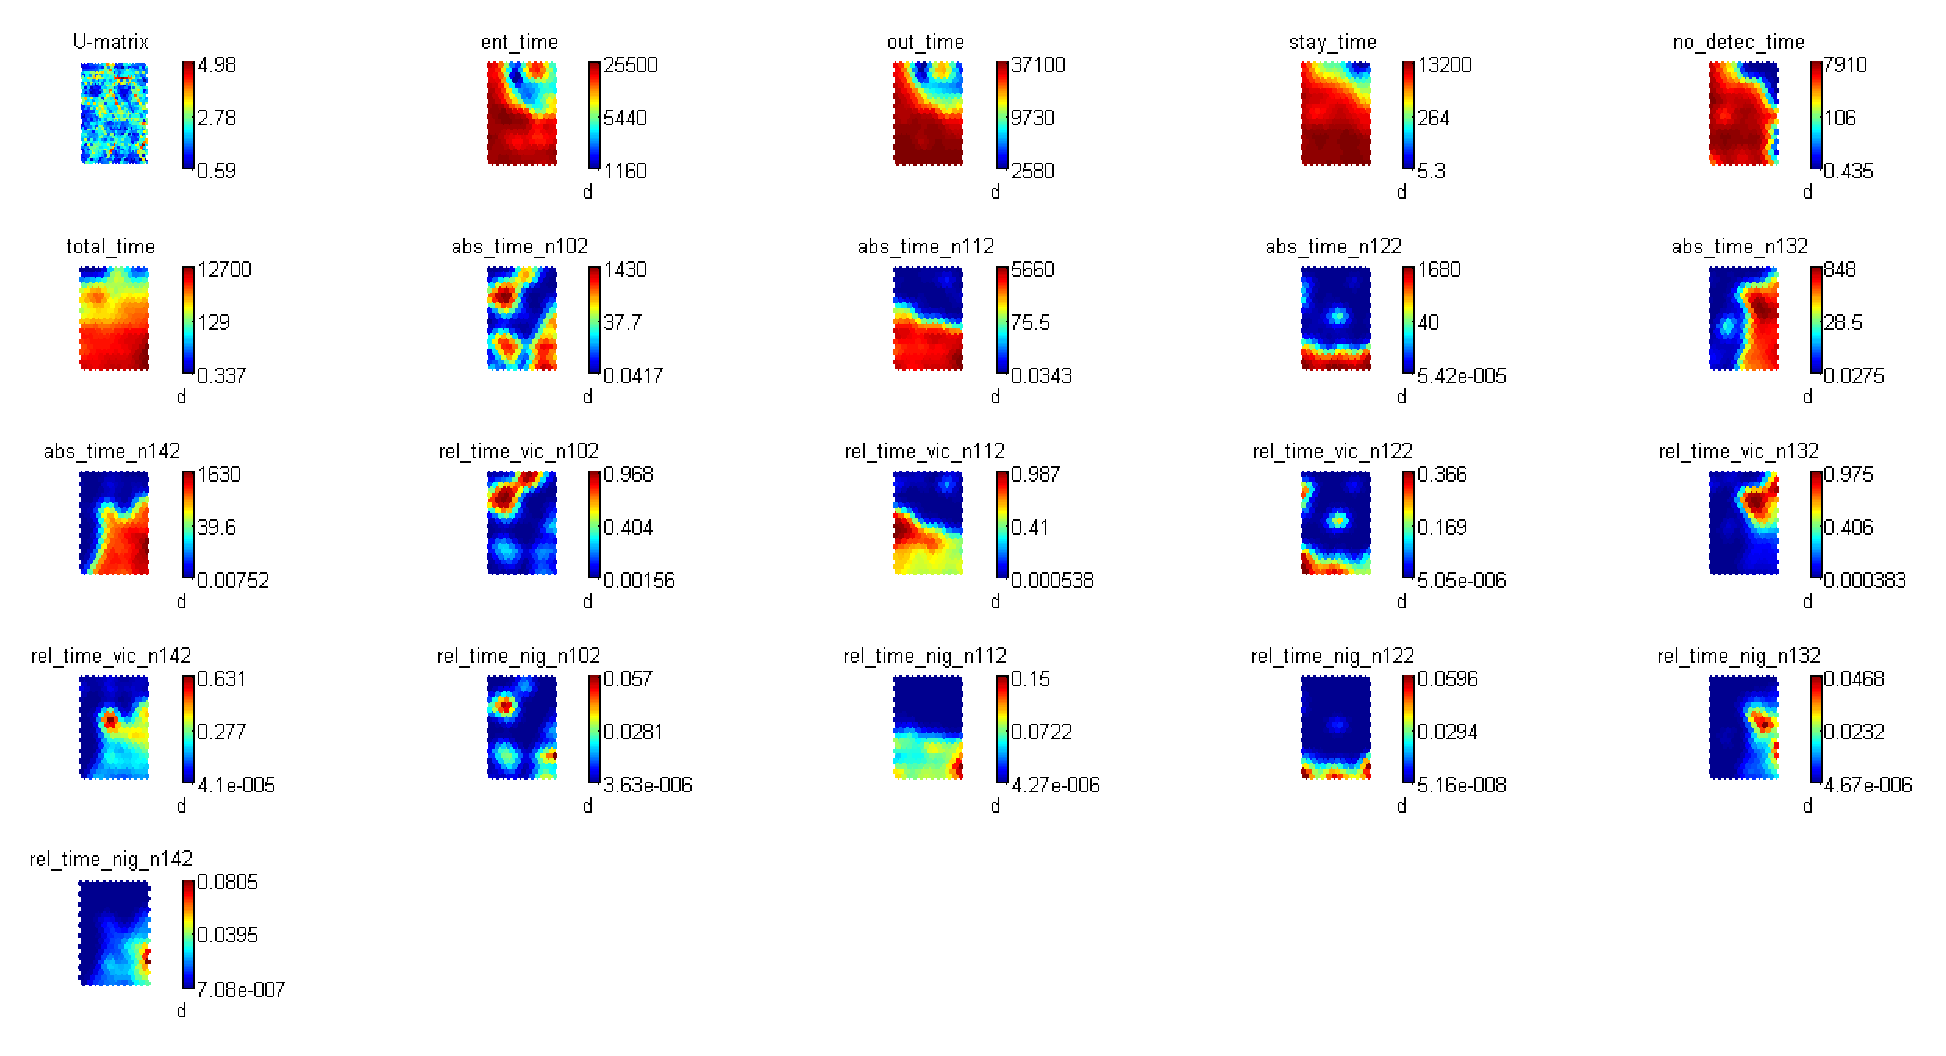
\includegraphics[width=14cm]{imgs/DISCO/som_disco_no_detec_0.eps}
%		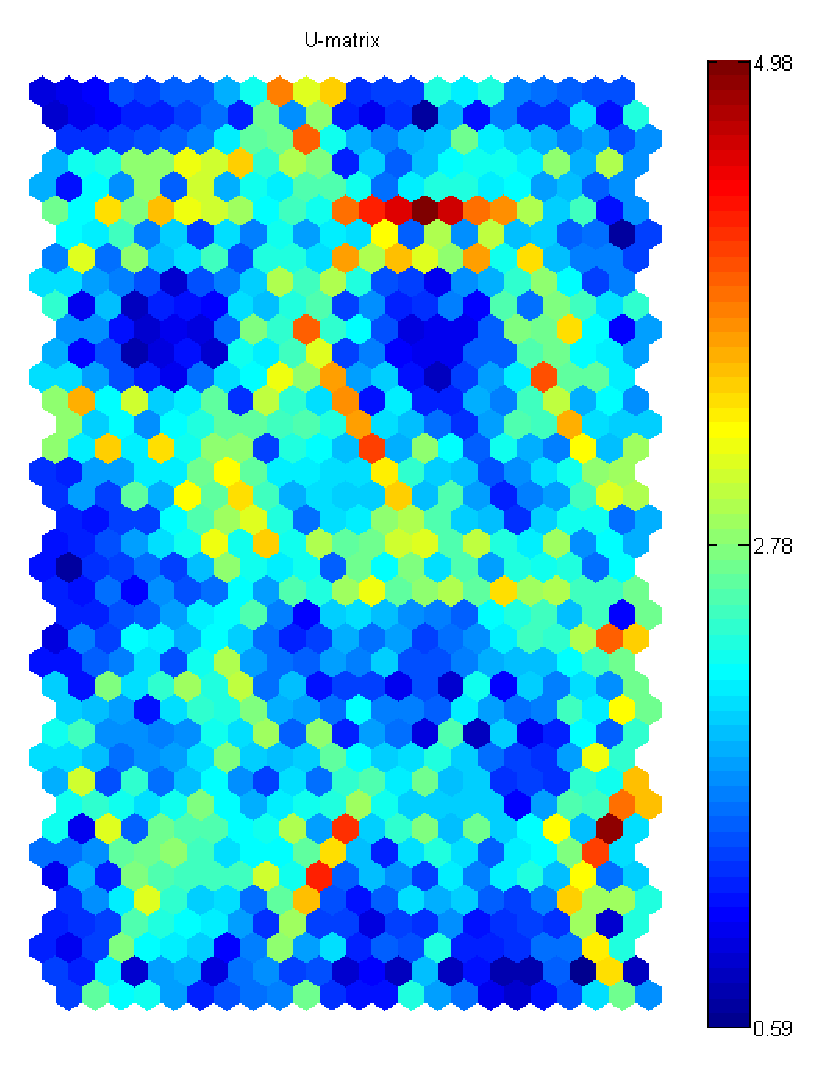
\includegraphics[width=8cm]{imgs/DISCO/umatrix_disco_no_detec_0.eps}
%		\caption{Detected devices in a night in the Discotheque scenario. Extracted features}
% Antonio - Ajustados los no detectados a 0
%		\label{fig:som_disco_no_detec_0}
%	\end{center}
%\end{figure}

\begin{figure}[!ht]
	\begin{center}
		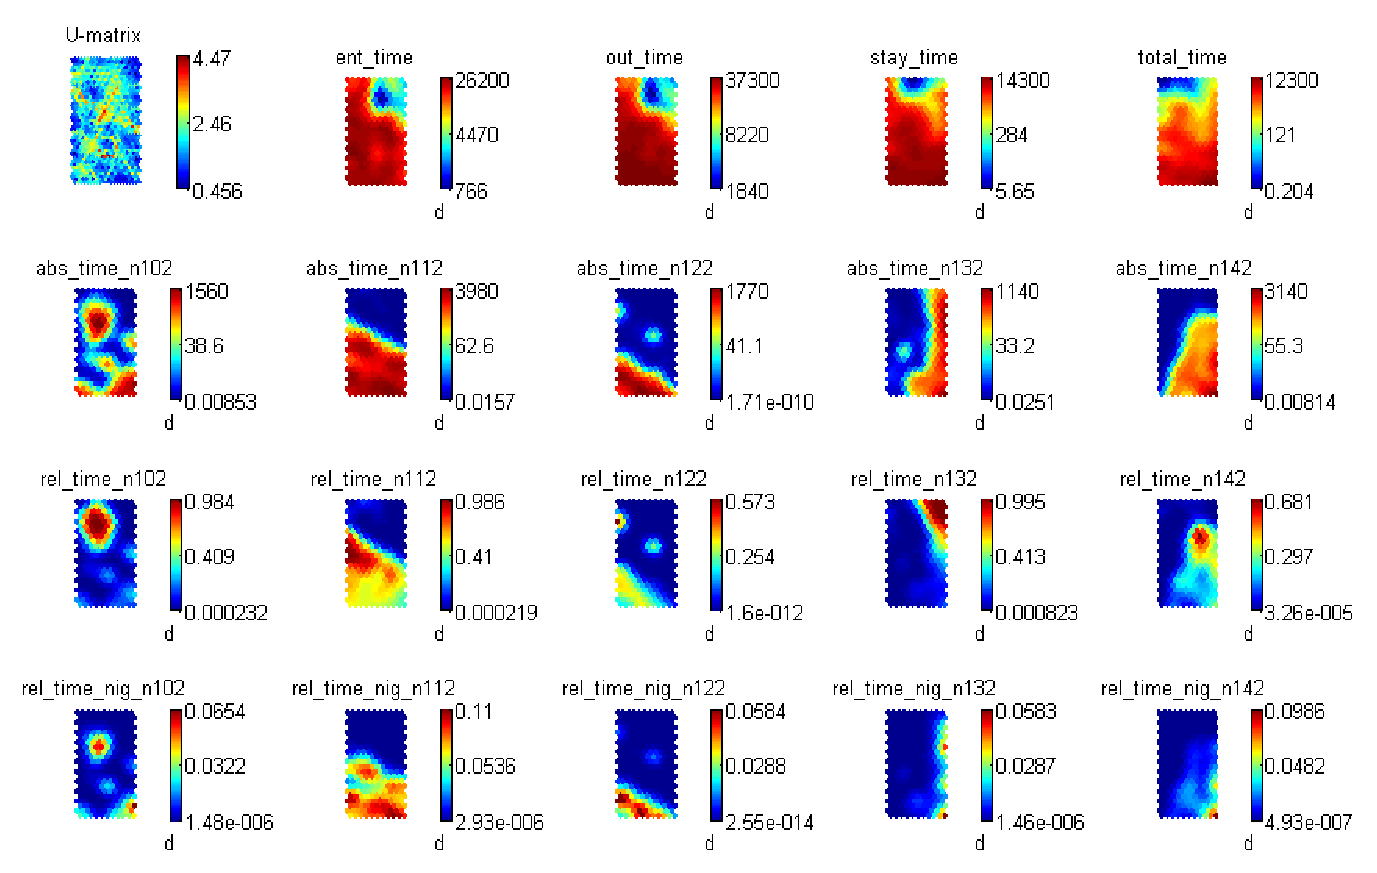
\includegraphics[width=12cm]{imgs/DISCO/som_disco_sin_no_detec.eps}
		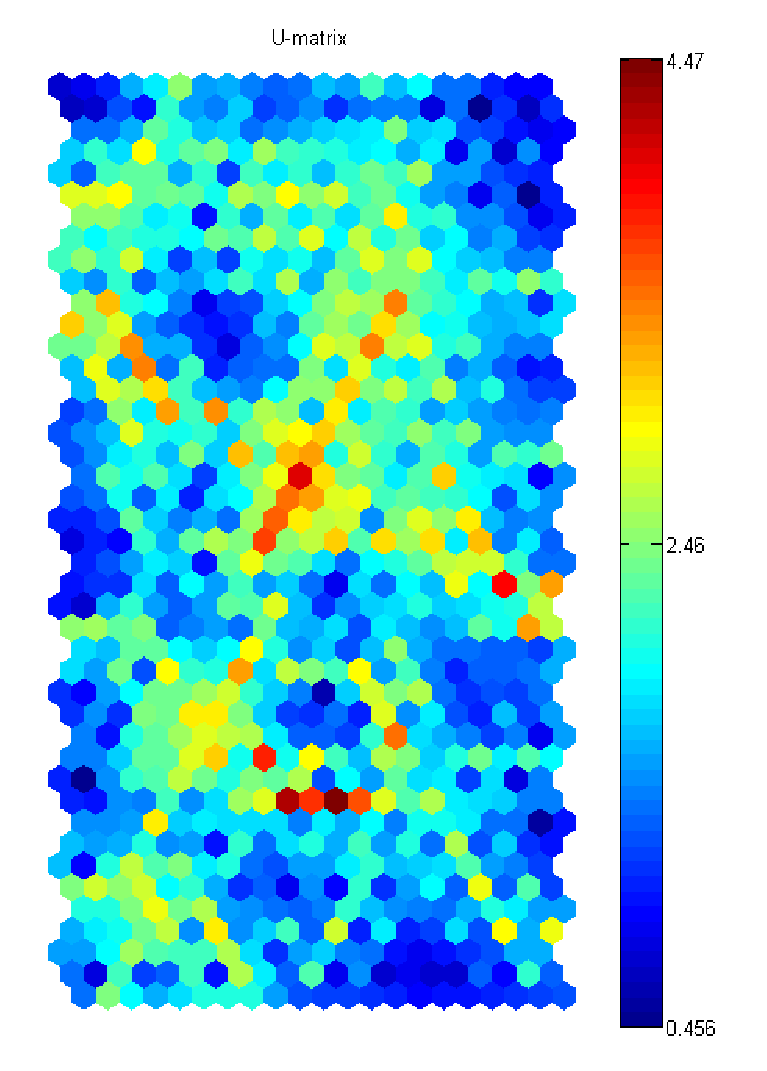
\includegraphics[width=6cm]{imgs/DISCO/umatrix_disco_sin_no_detec.eps}
		\caption{SOM + U-MATRIX Applied to the dataset of detected devices in a night in the Discotheque scenario. SOM Planes analysis (top) shows the extracted features described in Table \ref{tab:extracted_features_disco}}
% Antonio - Sin no detectados
		\label{fig:som_disco_sin_no_detec}
	\end{center}
\end{figure}

The results show that... *** COMENTARLOS ***
The problem is that there are no labels on the graph, so the interpretation cannot be as complete as it could... ***


In addition, another study has been conducted using SOM and U-MATRIX graphs. This time we want to analyse the \textit{recurrence of devices} to the discotheque, and their overall behaviour in the days they have come back. To this aim a new dataset has been composed, extracting those `events' of devices detected in more than two nights in two whole months.
Moreover, a similar set of features has been extracted for this experiment, as they are shown in Table \ref{tab:features_recurrence_disco}.

\begin{table}[htpb]
\centering
{\scriptsize
\begin{tabular}{lll}
\hline\noalign{\smallskip}
Variable name & Description & Type\\
\noalign{\smallskip}\hline\noalign{\smallskip}
\texttt{stay\_time} & Number of seconds the device has been in the disco & Integer\\
\texttt{abs\_time\_node\_X} & Number of seconds the device has been detected\\
& in every node X (from 1 to 5) & Integer\\
\texttt{relat\_time\_node\_X} & Percentage of time the device has been detected\\
& in every node X (from 1 to 5) & Float\\
\noalign{\smallskip}\hline
\end{tabular}
 \caption{Extracted features from gathered data in the discotheque. \label{tab:features_recurrence_disco}}
}
\end{table}

For each device, we have computed a sum of the amounts of diary time per monitoring node. Relative times have been also calculated as another set of features. There are 220000 monitored `events' and 2100 different devices, so this amount of patterns to cluster.

We have labelled the data using the number of different days every device has been detected (the recurrence rate).

The results on this study are shown in Figure \ref{fig:som_disco_recurrencia}.

\begin{figure}[!htp]
	\begin{center}
		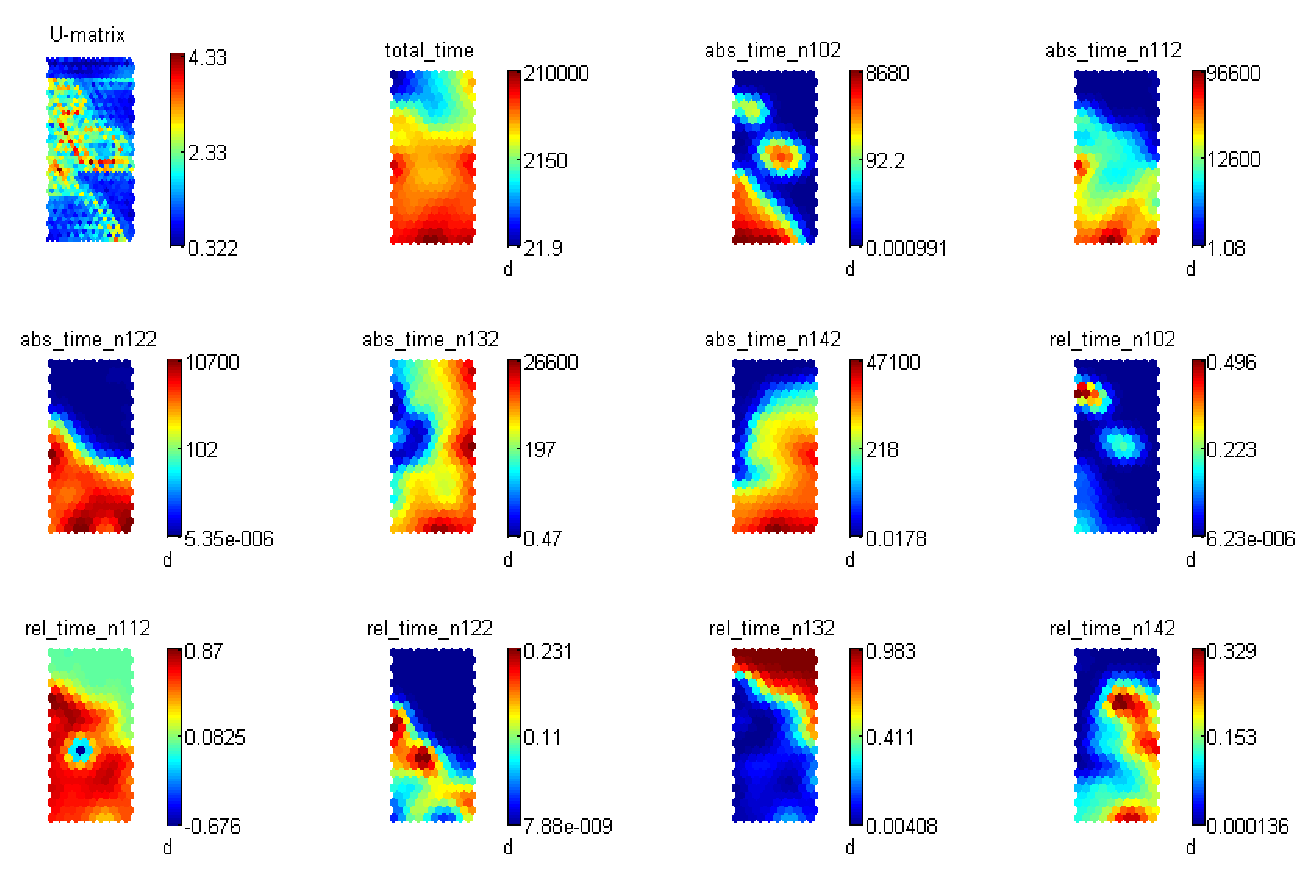
\includegraphics[width=11cm]{imgs/DISCO/som_recurrentes.eps}
		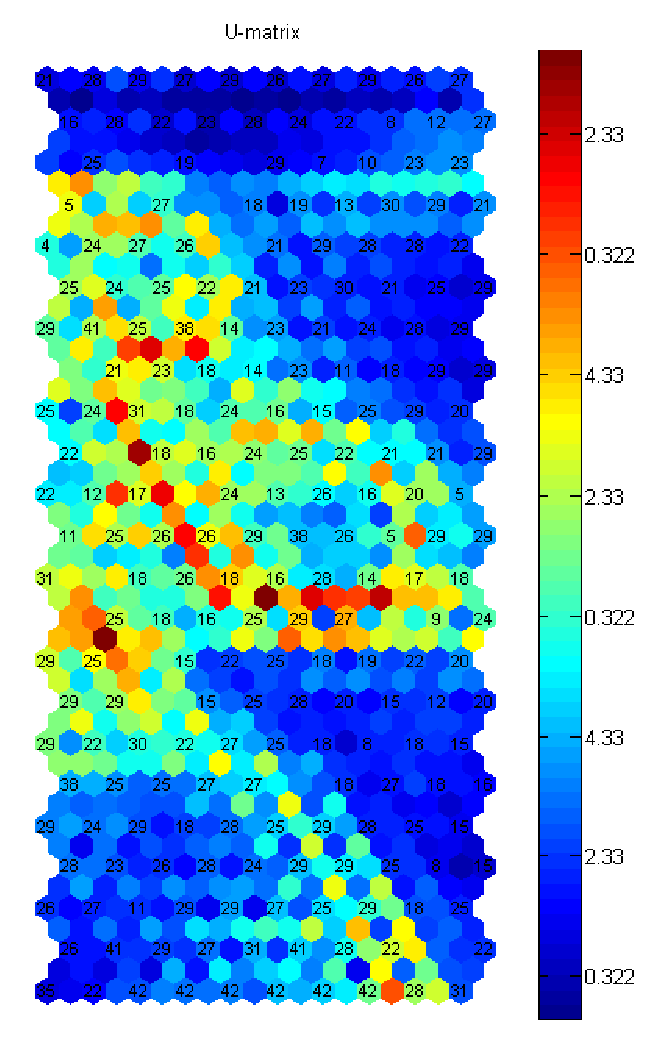
\includegraphics[width=6cm]{imgs/DISCO/umatrix_recurrentes.eps}
		\caption{Recurrence of devices in different days. The label is the recurrence rate (number of days the device has returned) of the majority in that neuron/BMU}
		\label{fig:som_disco_recurrencia}
	\end{center}
\end{figure}

As it can be seen in the U-Matrix every neuron (cell in the graph) has been labelled according to the class of the majority of the most similar input patterns. To this end the distance from every pattern to every neuron is computed considering their respective codevectors, the closest neuron to an input is named the best matching unit (BMU), and it is labelled with the pattern class (stage in this problem). Once the process has finished every neuron with more than one associated class finally displays the label with more occurrences.

*** COMENTAR RESULTADOS ***

- Comprobar aforo\\
- Aumentar seguridad\\
- Eficiencia energética y de personal o servicios (más medios en las salas más masificadas)\\
- Estudiar eventos particulares\\
- Estudios con objetivos de salud => gente que sale a la terraza (a fumar, supuestamente)


%----------------------------------------------------------------------------
%%%%%%%%%%%%%%%%%%%%  PEOPLE'S MOBILITY IN A BUILDING  %%%%%%%%%%%%%%%%%%%%%%
%----------------------------------------------------------------------------

\section{Analysing people's mobility in a building of the University}
\label{sec:etsiit}

In this section we will focus on people's mobility, as explained in Section \ref{sec:soa}, in a public building: the School of Informatics (ETSIIT) at the University of Granada. The building is studied as a proof of concept for the MOBYWIT sensor described in section \ref{sec:mobywit}. In order to monitor people flow, three devices have been placed in the three accesses to the building, as it can be seen on Figure \ref{fig:etsiit_map}.

\begin{figure}[!ht]
	\begin{center}
		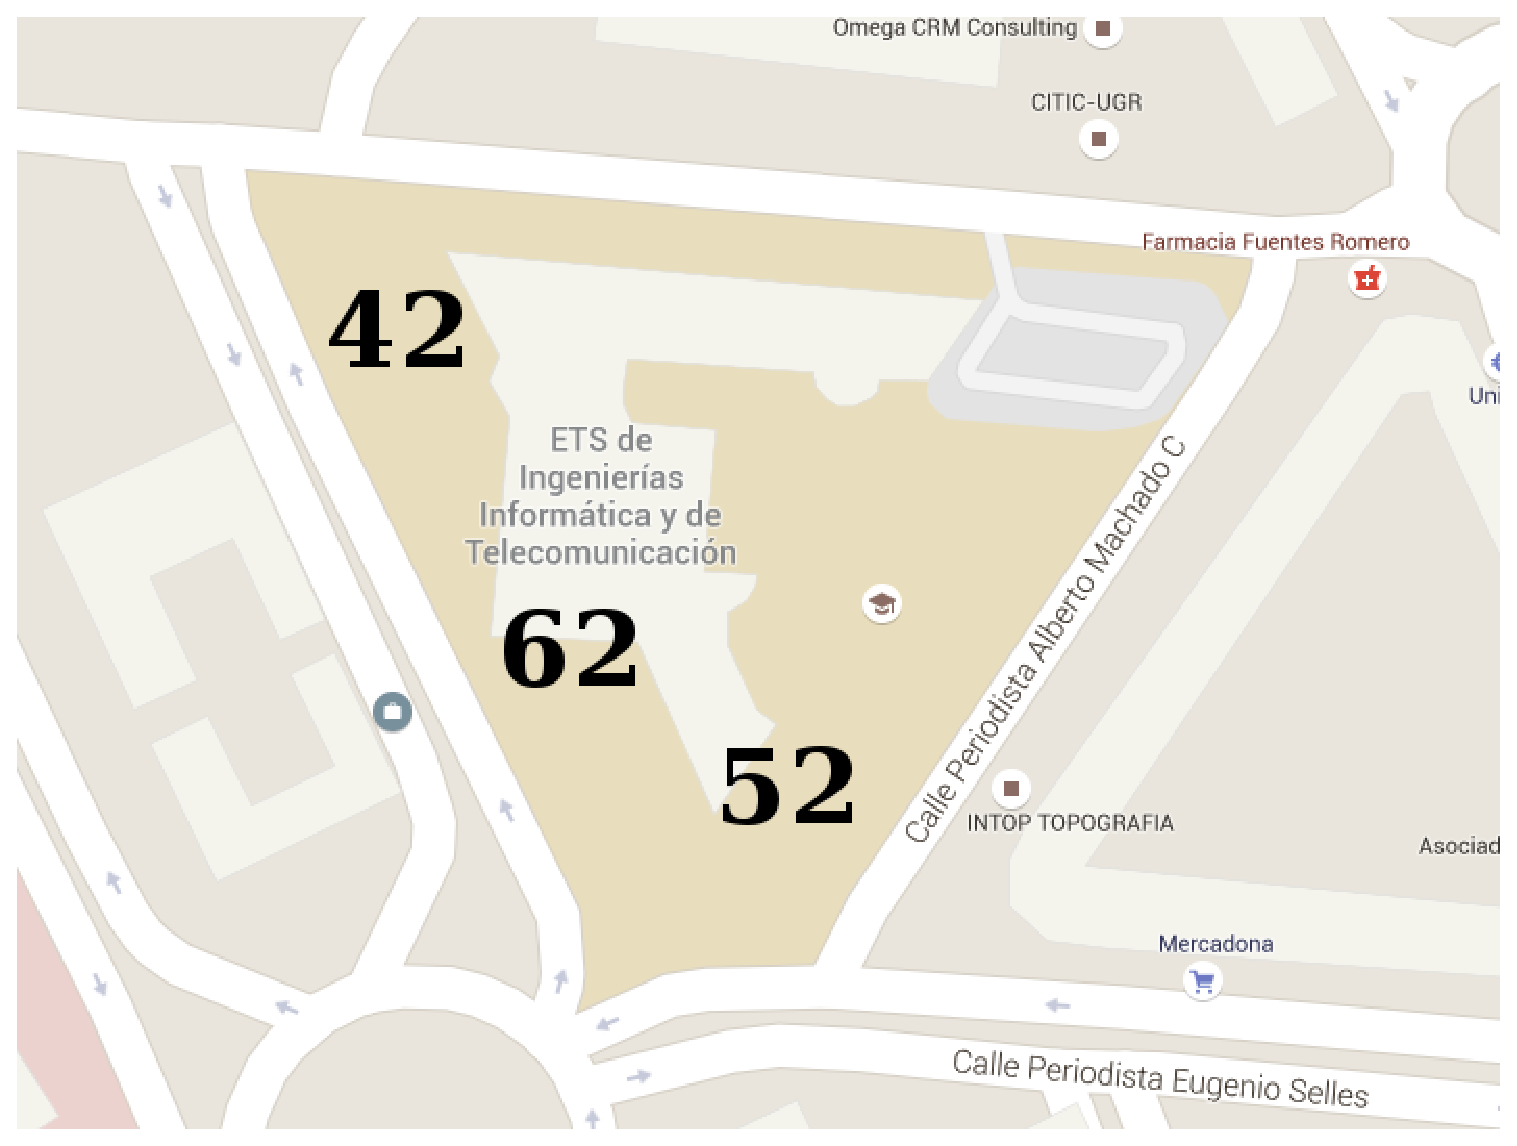
\includegraphics[height=4cm]{imgs/etsiit_nodes.eps}
		\caption{MOBYWIT devices location in ETSIIT}
		\label{fig:etsiit_map}
	\end{center}
\end{figure}

Since the devices can detect BT and WIFI signals from both the university staff and the students, two of them has been placed very close of the main access trying to distinguish staff (62) from students (52). The parking door (42) can only be used by the staff.

% please, ANTARES, help me a bit finishing the following paragraphs
The devices has been recording data for a few days only. With these data the origin-destination histogram that can be seen in figure \ref{fig:etsiit_io} has been created. A careful examination of this figure let us extract some conclusions.

\begin{figure}[!ht]
	\begin{center}
		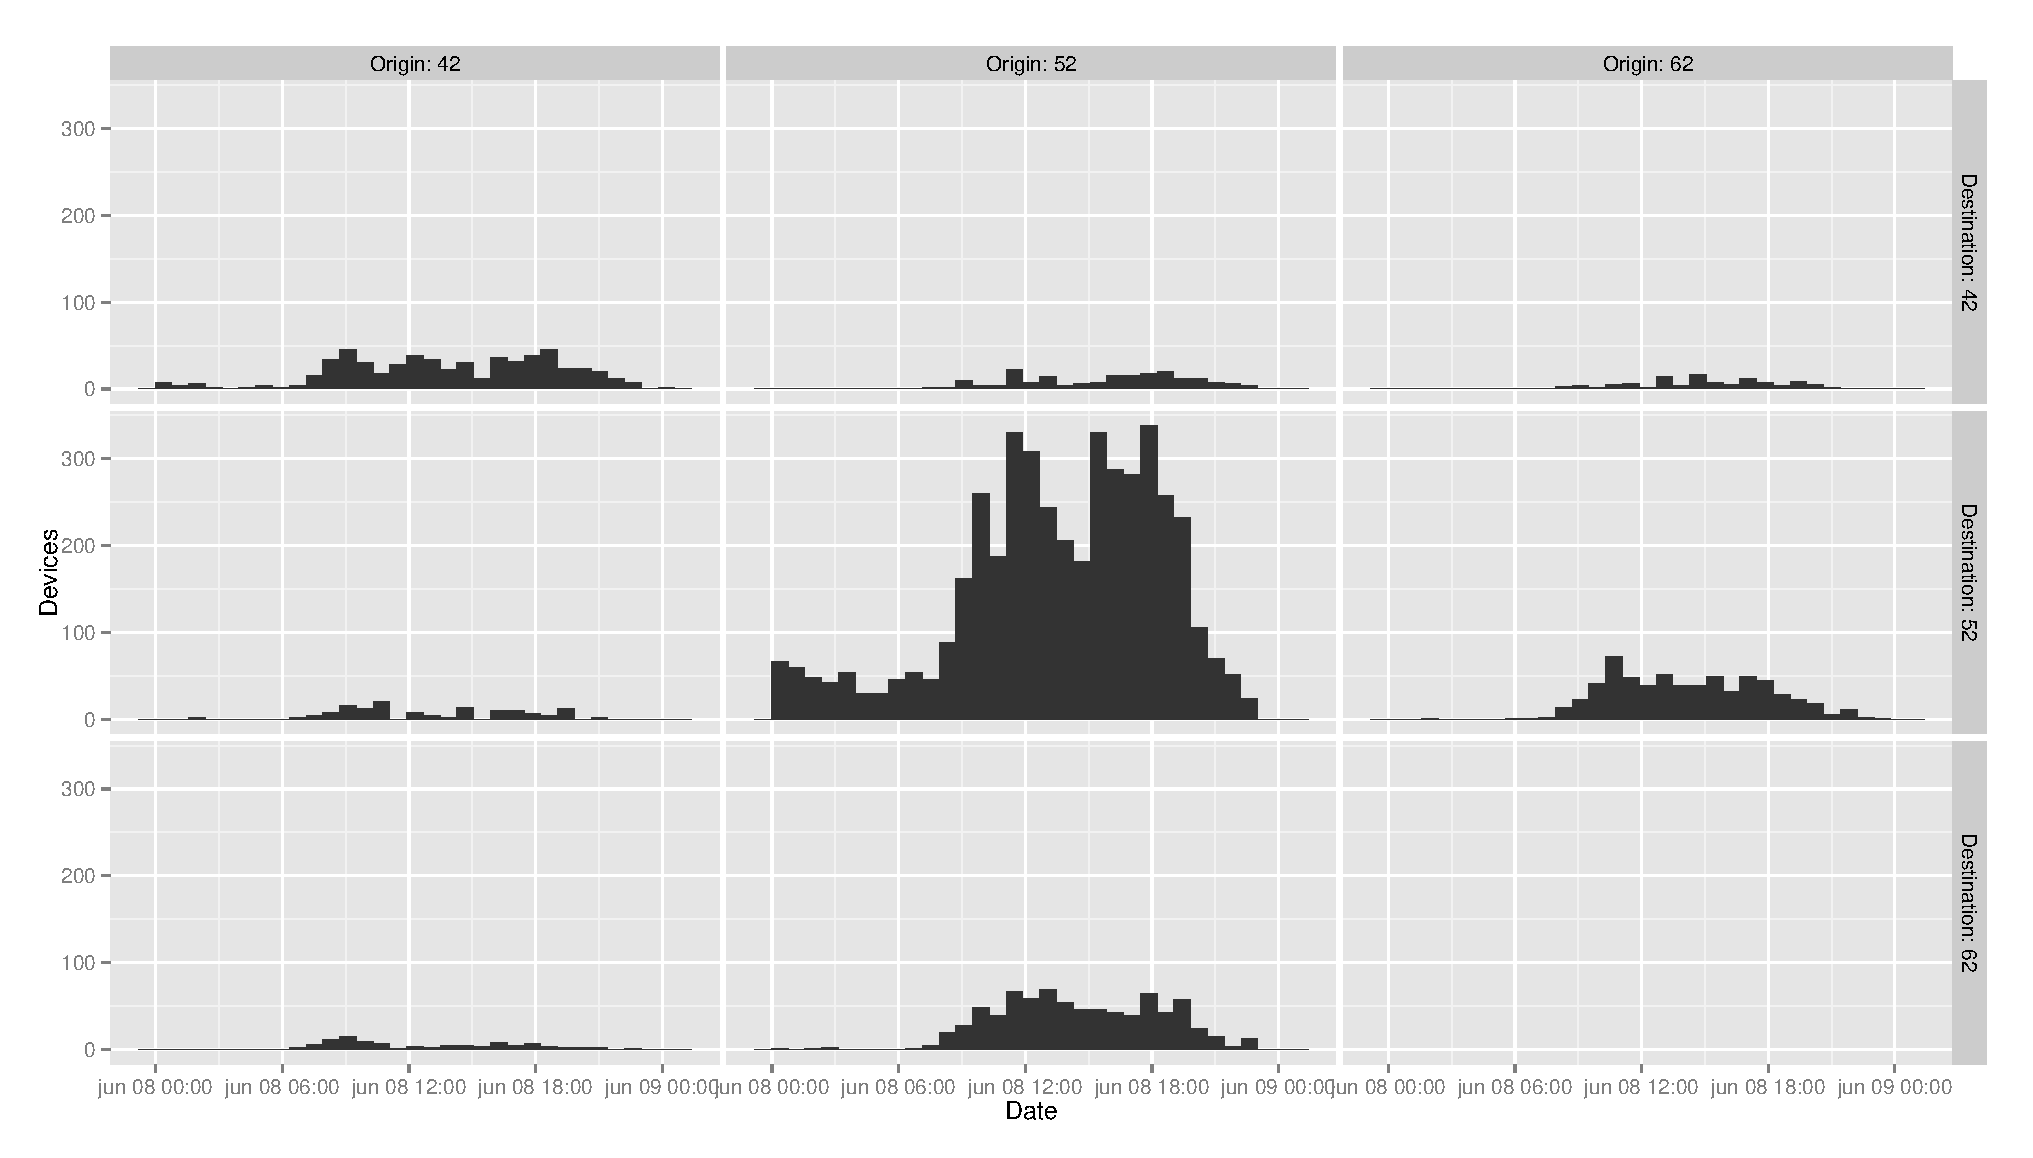
\includegraphics[width=\textwidth]{imgs/ETSIIT/etsiit_graph_origin-destination-histogram.eps}
		\caption{Origin/Destination histogram of people in ETSIIT}
		\label{fig:etsiit_io}
	\end{center}
\end{figure}

\begin{itemize}
\item Most people are students and they access the building through the students door (sensor 52 in figure \ref{fig:etsiit_map}). Most people get in and out by this door.
\item Professors and administrative staff seem to divide their way of getting in and out. They used the parking (sensor 42) as much as the main building door (sensor 62).
\item Many students go out by the main building (62) after a supposedly visit to a professor or an administrative.
%\item Some curious behavior has been discovered: some people who enter by door 42 exit by the parking (52). The only explanation possible is that the cafeteria and the lunch room are in the basement and they can get out without getting up one floor. %Antares - El sensor 52 es el de la puerta del aulario, no el del parking.
\item Why people getting in by main door (62) almost never go out by the same door? Most of them are students and go out by their door (52) at the end of the classes.
%\item We have failed to explain why not as many people who enter by the parking (42) leave the place by the same door. Cars can't be left there overnight.
\end{itemize}

With some additional sensors the people flow could be studied in a better way. Because with the three used many people can not be correctly interpreted as the right kind of visitor. The most interesting place for a new sensor is in the door of the classroom building at the north in the map.

Information gathered can be useful for the management of the building. When must heating be started? How many students are in class or just studying inside? Are there enough sits in the library? Are the doors in the right place? Many of this questions need a little more time to save enough data and answer them correctly.

%----------------------------------------------------------------------------
%%%%%%%%%%%%%%%%%%%%%%%%%%%   TRAFFIC in a HIGHWAY  %%%%%%%%%%%%%%%%%%%%%%%%%
%----------------------------------------------------------------------------

\section{Analysing the traffic in a highway}
\label{sec:traffic}

This section describes the experimental analysis of the data gathered by a 
different number of devices placed in national highways.

The main difference with respect to the other experimental scenarios is that, 
in this case, the detected devices are cars moving at higher speed. However, 
in this scenario we also count with the information provided by the Spanish 
traffic management agency, Direcci\'on General de Tr\'afico (DGT), which is 
collected using loop detectors. So, in this case, we have used real data in 
order to validate our approach by comparing the real number of vehicles which 
has passed a point, with the number of devices detected by MOBYWIT. Thus, a 
realistic \textit{ratio} between both numbers has been computed.

Six nodes have been placed along different roads in Andalusia (south Spain). 
Figure \ref{fig:nodosDGT} shows the identifiers of these devices and their 
exact location. These locations have been chosen because are the nearest   % nearest  or  closest  ???   [pedro] FERGU: el translate dice nearest por defecto, pero vamos, ni idea xD
ones to existent loop detectors monitored by the DGT, and also, they have 
Internet connection to allow the transmission of data to our server. 
There exist two groups of nodes: one in the province of Granada area 
(1010, 1020 and 1030) and the other in the road to M{\'a}laga (1040, 1050 and 1060).

\begin{figure}[htb]
	\begin{center}
		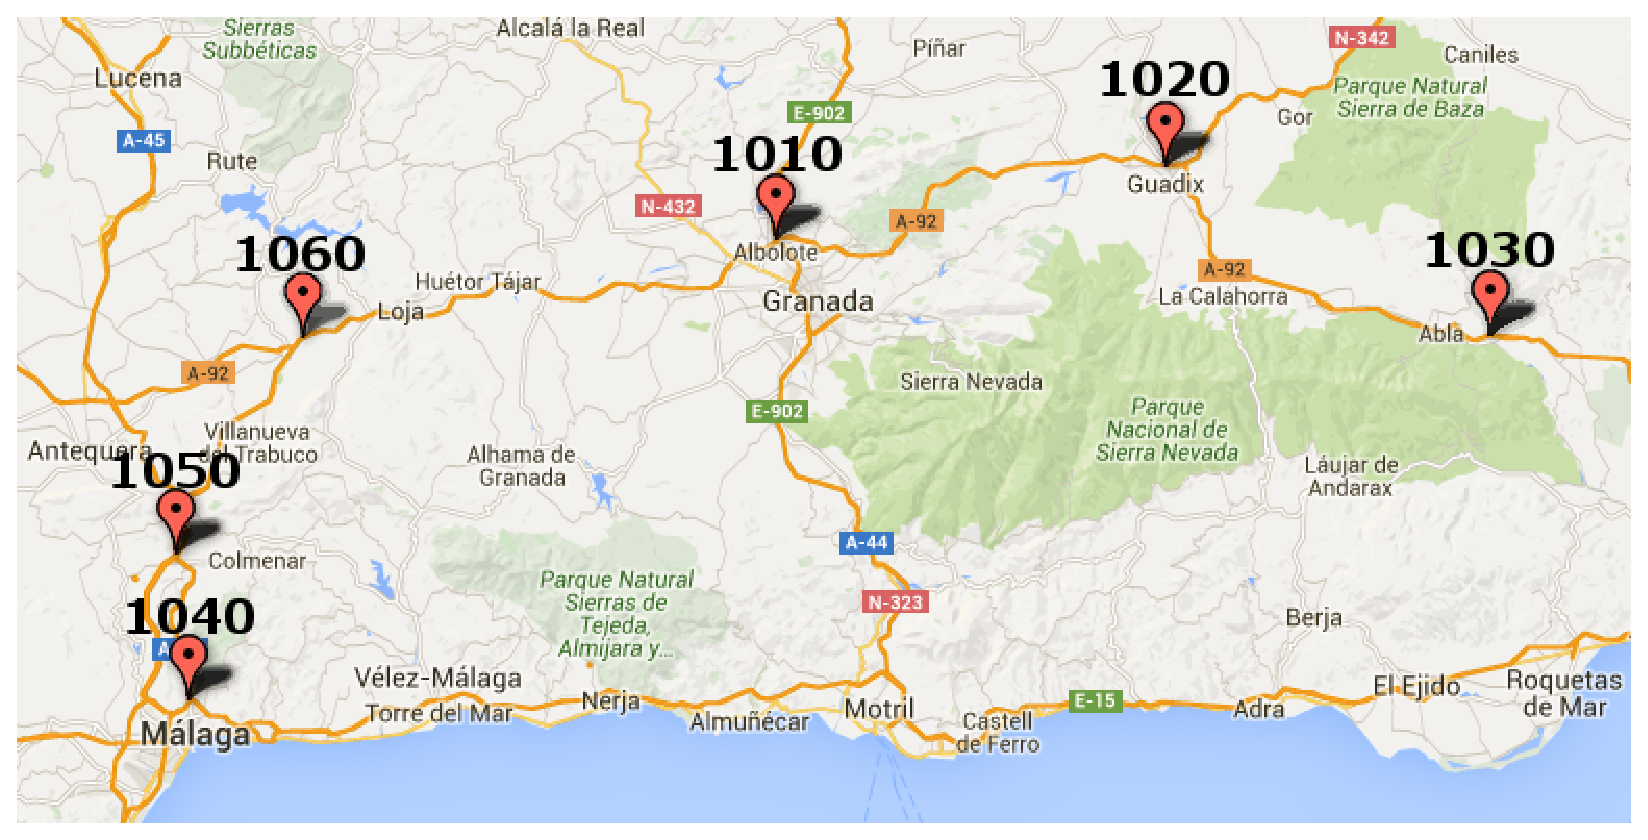
\includegraphics[scale=0.4]{imgs/nodos_dgt.eps}
		\caption{Location of MOBYWIT devices for the highway traffic scenario}
	\label{fig:nodosDGT}
	\end{center}
\end{figure}

In this section, several experiment will be conducted. First, an study on the velocity and driving behaviour taking into account the tracking capabilities of MOBYWIT will be presented. Also, different methods to extract a ratio between our gathered data and the real data provided by the DGT will be performed. Finally, a time series forecasting study will be performed. In order to compare the performance of the different methods, 9 frequently used error measures will be used in this section:
Mean Error ({\em ME}),
 Mean Squared Error ({\em MSE}),
 Root Mean Squared Error ({\em RMSE}),
 Mean Absolute Error ({\em MAE}),
 Mean Absolute Scaled Error ({\em MASE}),
 Median Absolute Error ({\em MdAE}),
 Median Absolute Percentage Error ({\em MdAPE(\%)}),
 Symmetric Mean Absolute Percentage Error ({\em sMAPE(\%)}), and
 Symmetric Median Absolute Percentage Error ({\em sMdAPE(\%)}).

Their different features, as well as their equations, can be found in Hyndman and Koehler's work ~\cite{RePEc:eee:intfor:v:22:y:2006:i:4:p:679-688}




\subsection{Driving behaviour}

Using the capability of the unique vehicle detection by MAC, we can calculate the passing frequency between nodes, and also, the travel time between them. Figure \ref{fig:dgtMatrixFrec} shows the frequency matrix between nodes. A time window for detection has been set to 2.5 hours (as it is a little more of the time between 1040 and 1030 according Google Maps). Results show that, patently, there are more repetitions between the nodes of the same continuous road branch. For example, between 1040 and 1050, as there exist a deviation to Seville before node 1060. This is clearer at the end of the week, where people come back to their villages/other cities to spent the weekends, and more repetitions are detected. Some repetitions have not been detected in the more separated nodes (for example, between 1040 and 1030), because shorter intercity routes exist following the coastline, instead the interior.

%\begin{enumerate}
%    \item Matriz de E/S con frecuencia
%    \item Matriz de E/S con tiempos
%    \item Grafica de Velocidades
%\end{enumerate}


\begin{figure}[htb]
	\begin{center}
		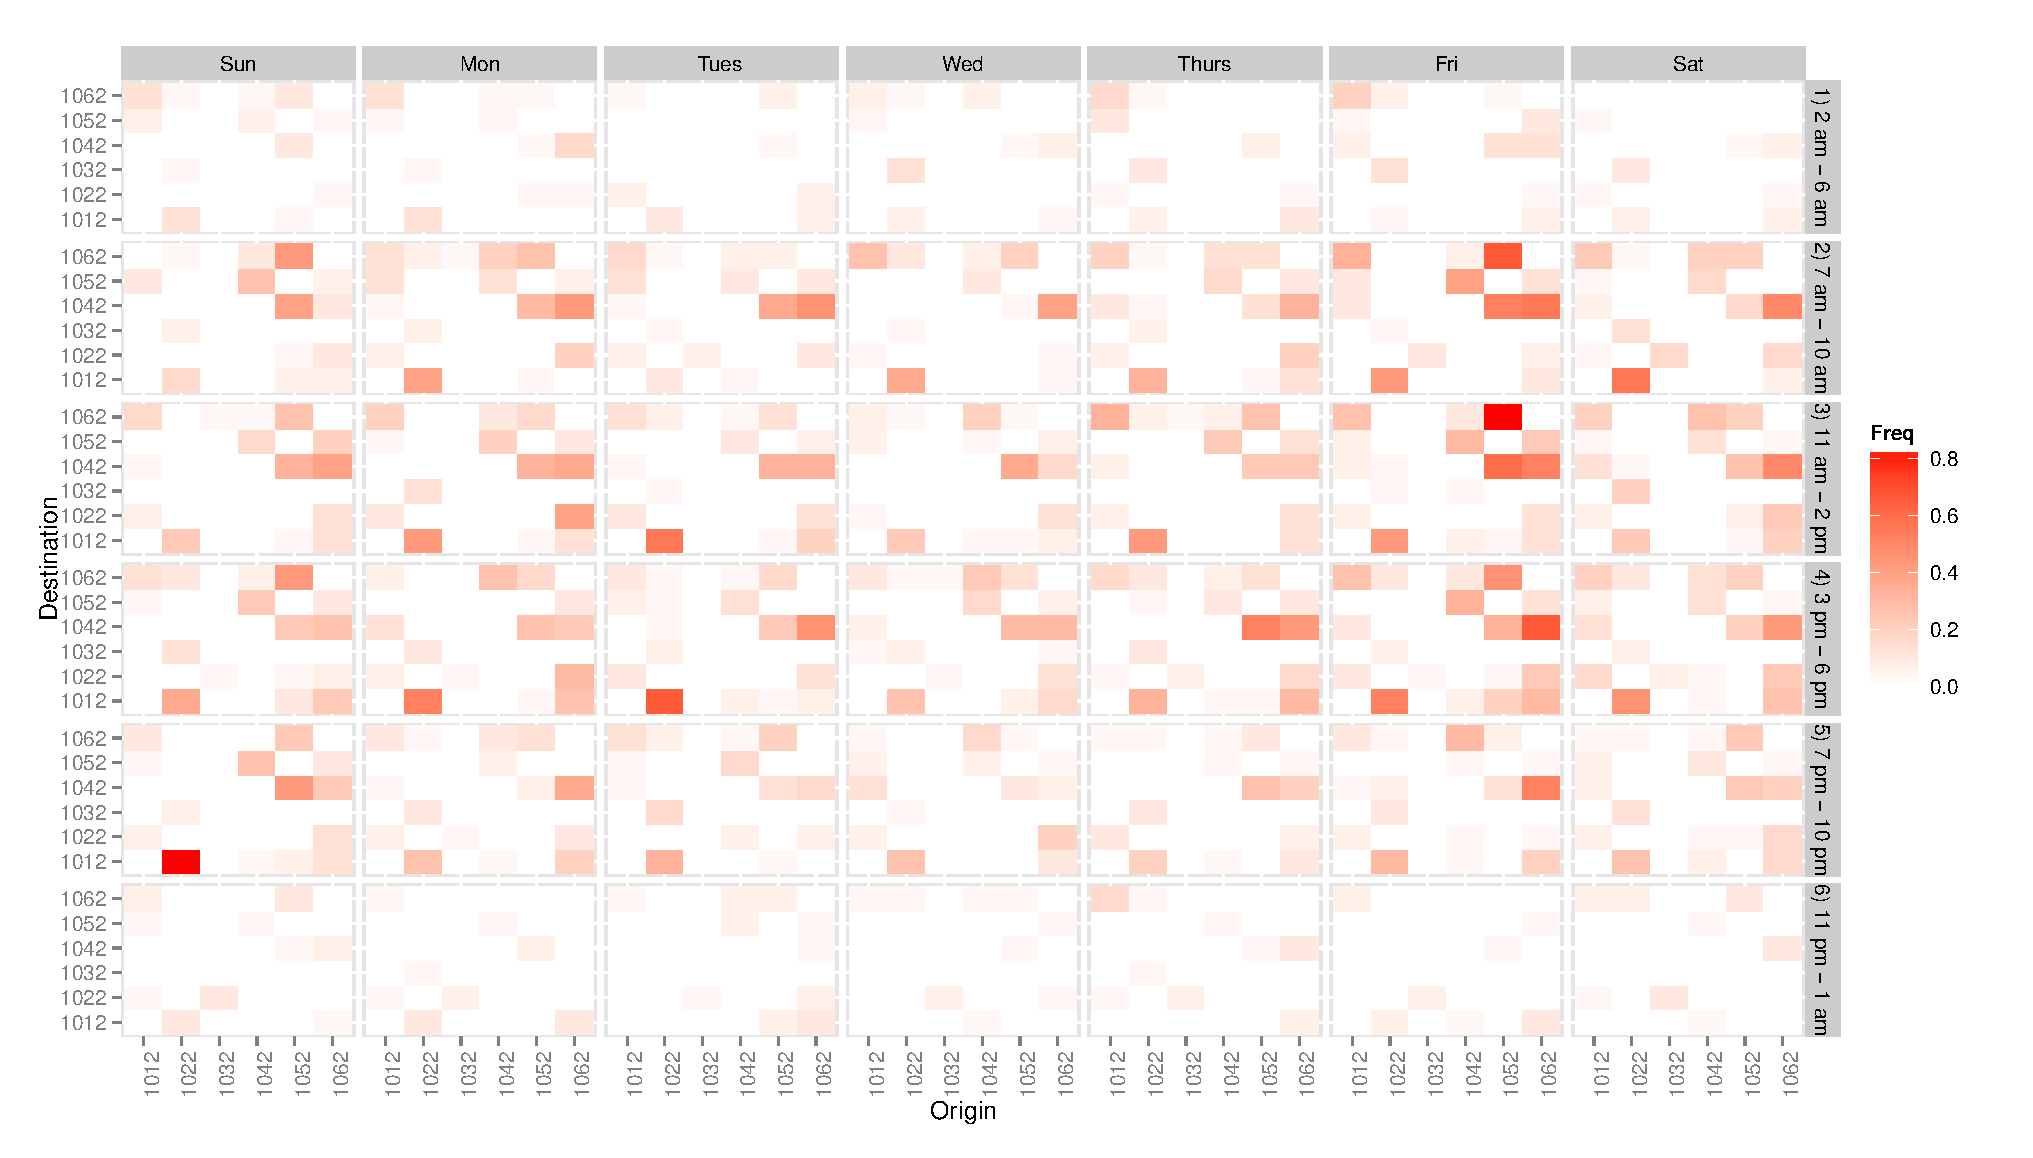
\includegraphics[scale=0.4]{imgs/petra_matrix_freq.eps}
		\caption{Frequency between nodes, detecting the unique vehicle identifiers by our MOBYWIT devices. Every day is grouped in blocks of 4 hours.}
	\label{fig:dgtMatrixFrec}
	\end{center}
\end{figure}

Using the time when each repetition has been detected we can also calculate average speed velocity during the week. Figure \ref{fig:dgtMatrixTime} shows the detected times between nodes, in blocks of 4 hours, during the week. Largest travel times are detected between more separated nodes. As in previous figure, time between more separated nodes is not tracked because shorter paths between cities exist. HABLAR MAS DE ESTOS DATOS

\begin{figure}[htb]
	\begin{center}
		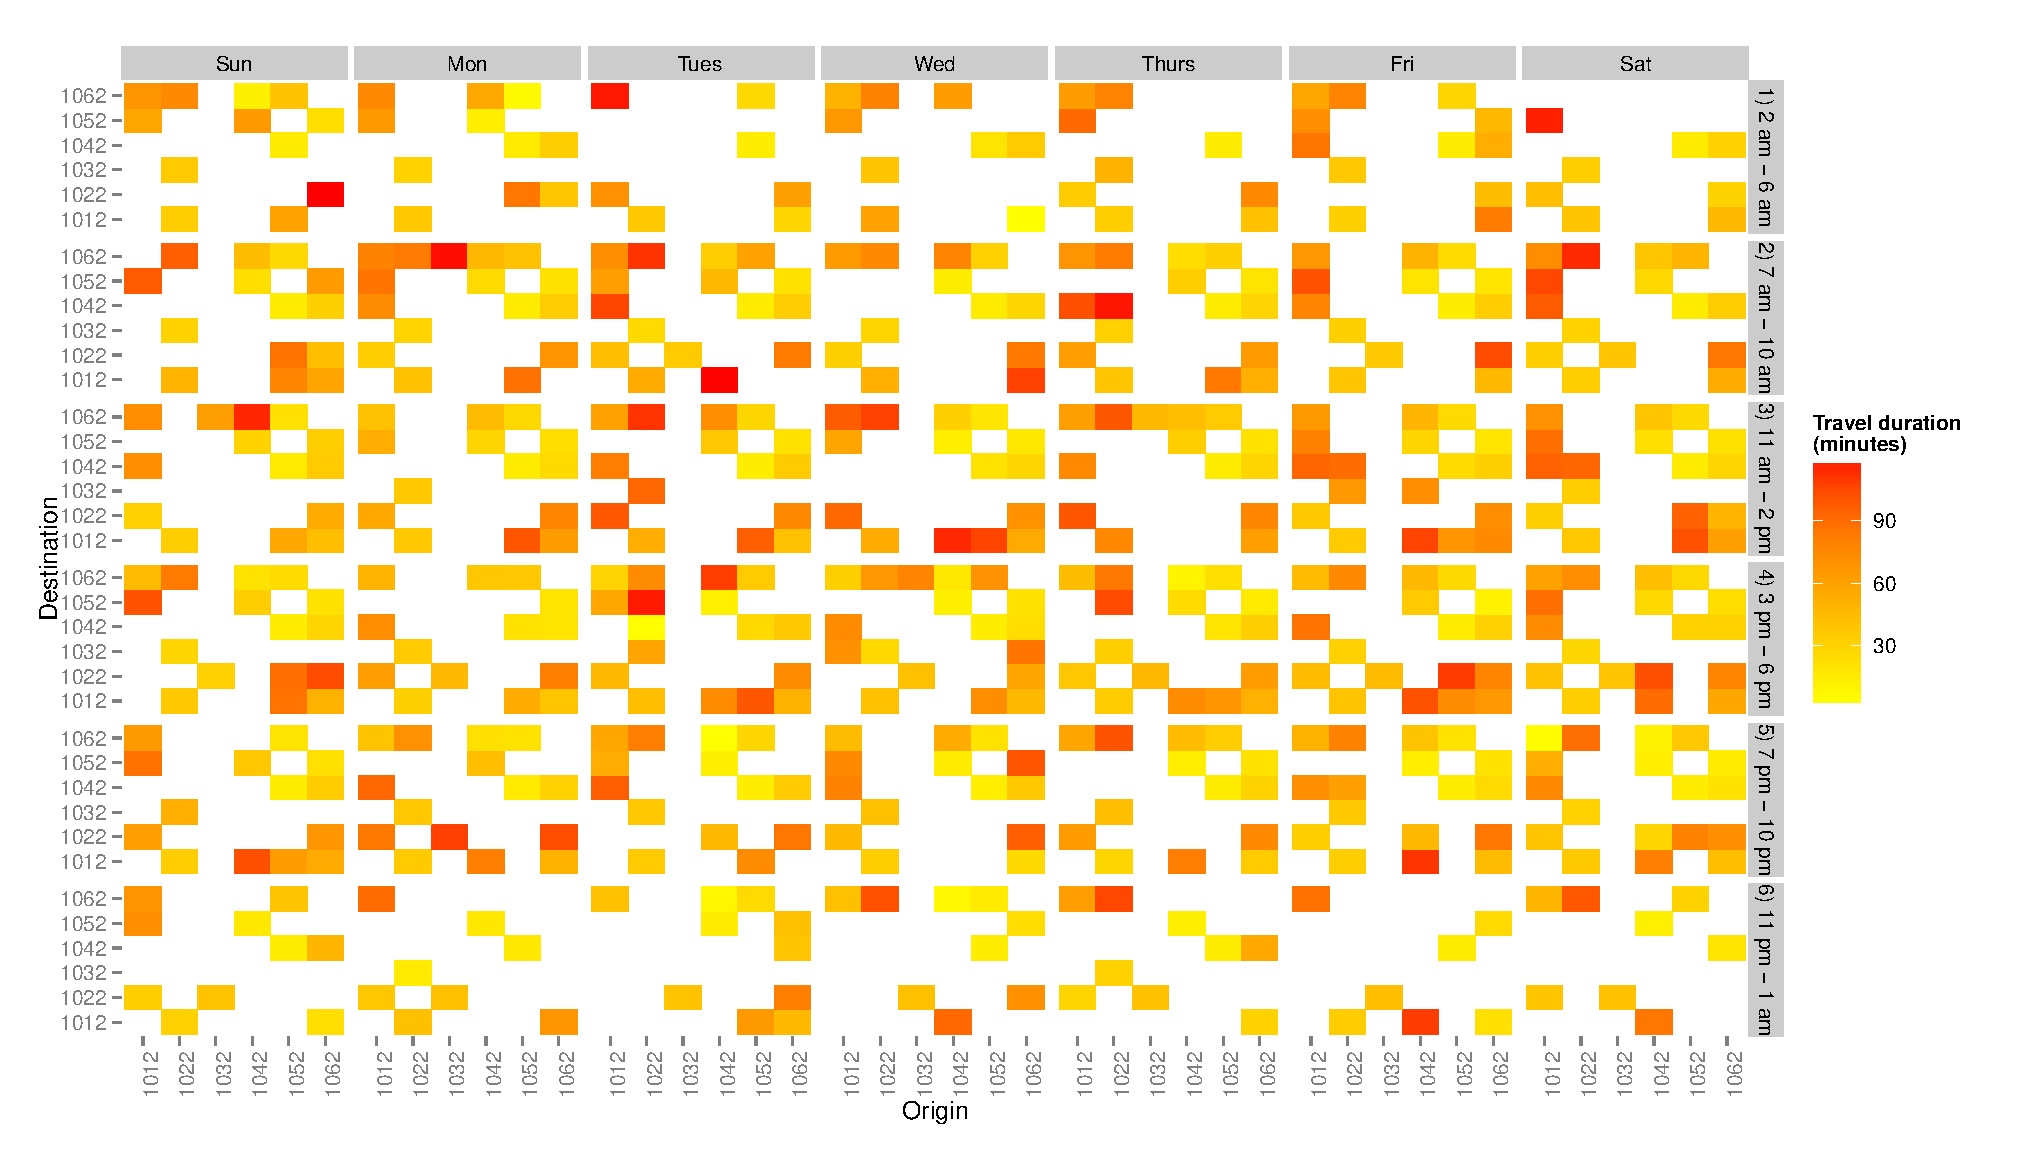
\includegraphics[scale=0.35]{imgs/petra_matrix_travelDuration.eps}
		\caption{Average time between nodes, detecting the unique vehicle identifiers by our MOBYWIT devices. Every day is grouped in blocks of 4 hours.}
	\label{fig:dgtMatrixTime}
	\end{center}
\end{figure}


\subsection{Data validation using other sources of data}

Different metrics will be used to obtain a correct correlation between the number of detected devices and the real number detected by the loop detectors. To simplify the data analysis and discussion only the data of one node (1010) is shown.

\begin{itemize}
\item {\em Total ratio}: ratio between the total number of vehicles detected by the DGT and the total number of vehicles detected by our device.
\item {\em Mean ratio}: as the maximum granularity of the data provided by the DGT is 15 minutes, the sum of all ratios between the DGT data and our data in each 15 minutes section has been divided by the total number of sections to calculate the average.
\item {\em Median ratio}: instead the average ratio as in previous metric, this one uses the median of all ratios.
\item {\em Mean by quarter ratio}: this metric calculate a vector of ratios separated by quarter of hour during the day, instead obtaining a global ratio for all data. An average ratio per quarter per hour in the vector is calculated taking into account all the ratios of that quarter during all the days we have data.
\item {\em Median by quarter ratio}: as in the previous metric, this one uses a vector of ratios per quarter of hour, but every element is calculated using the median, instead the average.
\end{itemize}


Table \ref{tab:ratiosDGT} shows the obtained ratios. *** COMENTARLOS ***

\begin{table}[htb]
\centering
\resizebox{12cm}{!}{
\begin{tabular}{|l|l|l|l|l|l|}
\hline
			 &RATIO	  & MAE    &   MAPE   & MSE    & RMSE \\
 \hline
Total Ratio  & 17.230 &   60.373 & 36.265 & \textbf{7371.579}  & \textbf{85.857} \\
Mean Ratio   & 20.792 &   72.323 & 43.443 & 11216.070 & 105.905 \\
Median Ratio & 18.2 &    62.454  & 37.515 & 8060.136  & 89.778 \\
Median By Quarter of Hour Ratio & Depends on the hour  & \textbf{58.326} & \textbf{35.035} & 7617.613 & 87.278 \\
Mean By Quarter of Hour Ratio &   Depends on the hour  & 66.791 & 40.120 & 9890.978 & 99.453 \\
\hline

\end{tabular}
}
\caption{Different ratios between the DGT data and the data gathered by MOBIWIT in node 1010.}
\label{tab:ratiosDGT}
\end{table}


Figure \ref{fig:dgtRatios} shows the number of devices of the node 1010, applying the chosen correction ratio. As it can be seen, certain correlation exist. However, different peaks appear in the figure, being those elements the product of detecting few devices in comparison with the DGT.



\begin{figure}[htb]
	\begin{center}
		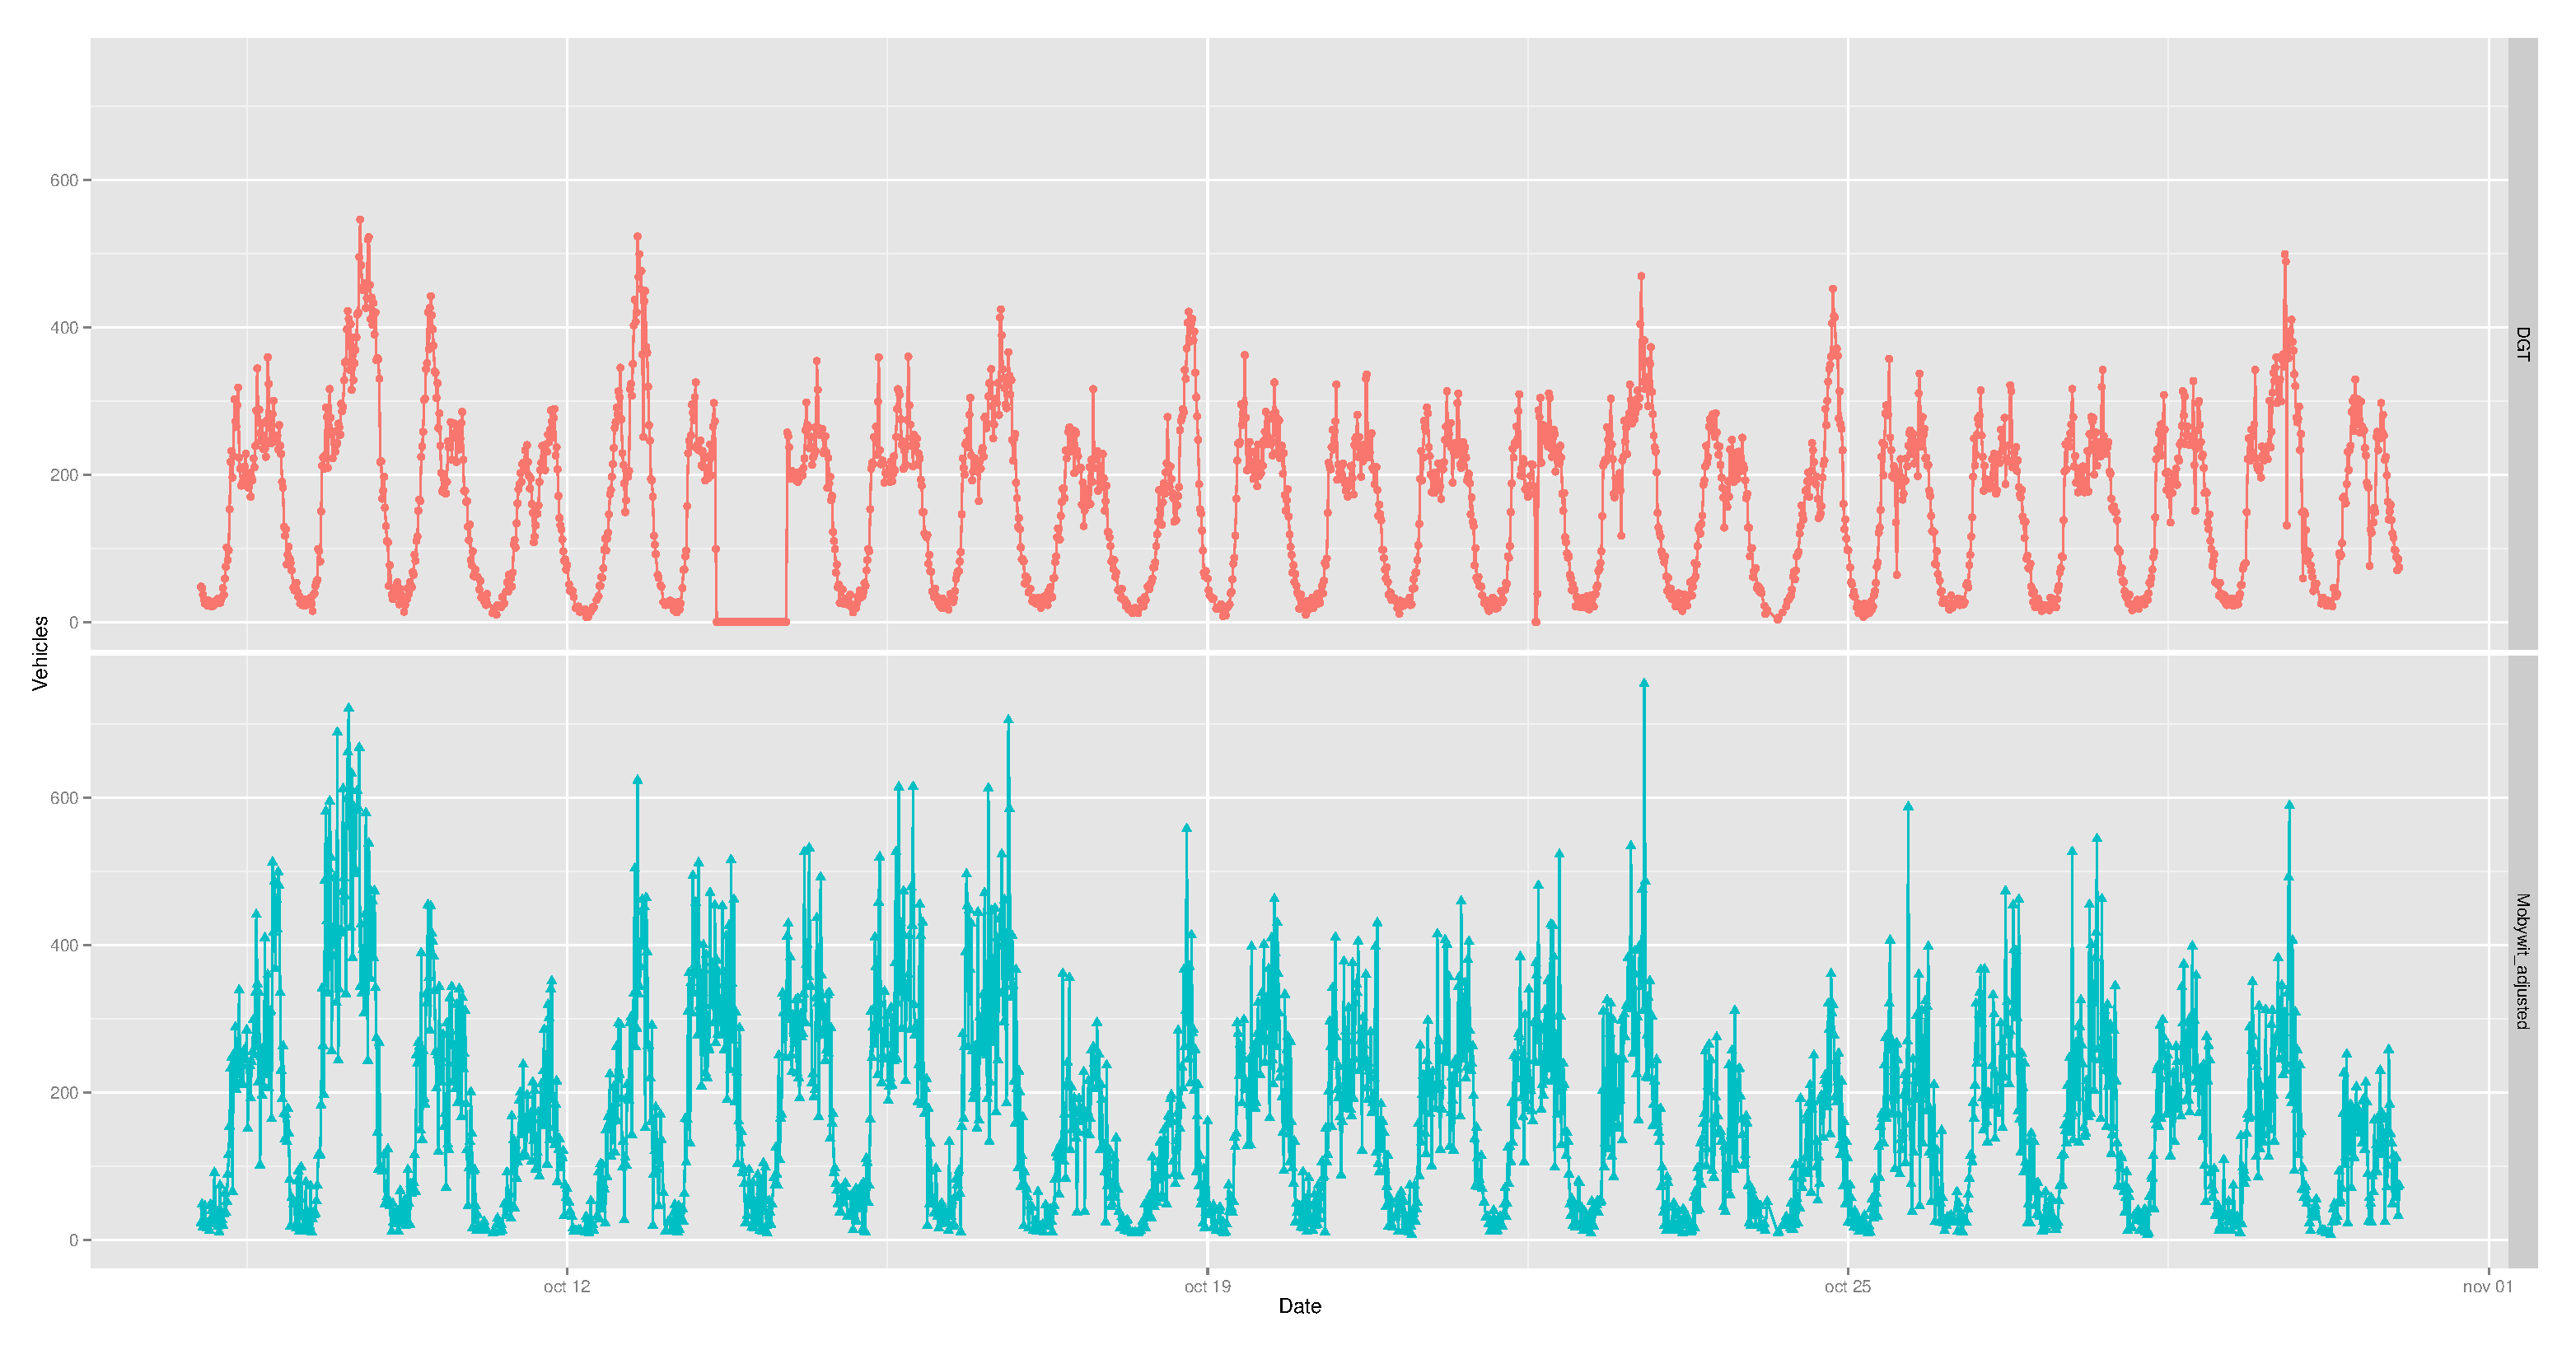
\includegraphics[scale=0.4]{imgs/petra_graph_DGT-Mobywit-mended.eps}
		\caption{Devices detected by DGT and detected by our device (node 1010) applying the correction ratio (median by quarter). Note: no DGT data available during Octuber 14th.}
	\label{fig:dgtRatios}
	\end{center}
\end{figure}

\subsection{Traffic forecasting}
\label{sub:ts_forecasting}
Capturing data about traffic in a highway worth not only for describing its current situation, but also for forecasting future conditions. In this sense, counting the number of cars that have passed for a given point in a given time can be considered as a time series, allowing the use of automatic tools to perform forecasting.

For this work, four methods (three widely used time series forecasters, and one control method) have been used to, automatically, predict the number of cars that will pass in the next period. These methods are included in the forecast package ~\cite{Hyndman08automatictime} of the R program~\cite{R:Bloomfield:2014}, and are the following:

\begin{itemize}
\item {\em Exponential smoothing state space model (ETS)~\cite{ETS:2008}}: Represent a set of methods that decompose the time-series in three different characteristics: error, trend and seasonal, modeling each one with a given equation. The forecasted values are obtained joining the previous equations by addition or multiplication. The corresponding function in the forecast package builds the different models included in the ETS set, and select the one with the best according to the Akaike's Information Criterion (AIC)~\cite{Akaike1973}.
\item {\em ARIMA~\cite{BoxJenk}: This well known method, due to Box and Jenkins } integrates autoregressive (AR) and moving average (MA) models in a three-stage iterative cycle. The phases of every cycle consist of: identifying the time series, estimating of the model's parameters, and verifying the built model. Briefly, every model is defined as a sum of $p+q$ terms. The first $p$  terms are defined by $p$ past values, any of them multiplied by a coefficient; while the last $q$ terms represent the moving averages, also multiplied by their own coefficients.
\item {\em Theta~\cite{Assima2000}}: This univariate forecasting method is based on modifying the local curvature of the time-series, after having applied a second difference to the data. It decomposes the original time series into several modified ones, which are separately extrapolated so that they have to be combined in order to provide the forecasting.
\item {\em Mean}: This is the control method. The future values are computed as the mean of the previous ones.
\end{itemize}

The data used for the experiments are the ones provided by the node 1010 starting on 12-Oct-2015, 00:00 hours, and finishing on 31-Oct-2015, 23:45 hours, i.e., three entire weeks less one day (there exist no data for November, the first). As data is aggregated every 15 minutes, this means the time-series was composed of $20(days)*24(hours)*4(quarters)=1920$ values.



Table ~\ref{tab:forecasting} shows the values for the ten used measures computed over $576$ values, the ones corresponding to the last 6 days (i.e., $30\%$ of the data). The horizon has been set to 1, so that, in order to forecast any given moment all the previous real known data were used to build and train the models and, after this, the next value was forecasted. This way, the problem has been faced as a simulation of what could happen in a continuous system in which new real data where received every 15 minutes so that forecasting models could be also continuously adapted.

As results show, ETS, ARIMA and Theta behave clearly better than the control method. The differences between the three considered methods are, almost nonexistent. In any case, ETS yields the lowest values in six of the measures been used so that, a priori, it could be considered the best candidate to be chosen as the preferred method to forecast this kind of time-series. Figure \ref{fig:forecasted-values} depicts the values forecasted by ETS comparing them with the expected ones.

\begin{figure}[!ht]
	\begin{center}
		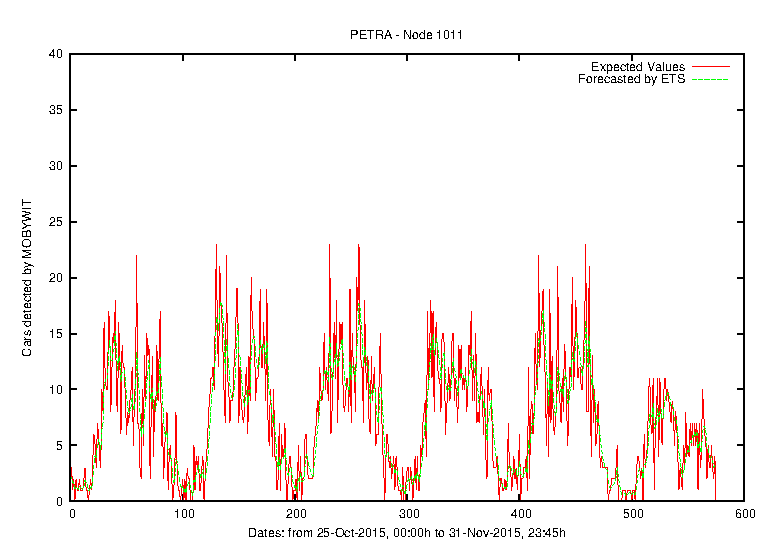
\includegraphics[width=14cm]{imgs/PETRA/forecasting-PETRA-1011.eps}
		\caption{Expected vs forecasted number of cars in node 1011, according to MOBYWIT's records. Forecasted values are provided by smoothing state space model (ETS). }
		\label{fig:forecasted-values}
	\end{center}
\end{figure}

\begin{table}
\centering
%\resizebox{12cm}{!}{
\begin{tabular}{|c|c|c|c|c|}
\hline
Measure vs Method &Mean &ETS &ARIMA &Theta\\
\hline
ME &$0,6631$ & $0,0059$ & $0,0043$ & $\textbf{0,0034}$\\
MSE &$28,5711$ & $\textbf{13,0194}$ & $13,2775$ & $13,0421$\\
RMSE &$5,3452$ & $\textbf{3,6082}$ & $3,6438$ & $3,6114$\\
MAE &$4,4611$ & $\textbf{2,7106}$ & $2,7409$ & $2,7126$\\
MASE &$4,7226$ & $\textbf{1,0128}$ & $1,0822$ & $1,0599$\\
MdAE &$1,4009$ & $\textbf{0,8512}$ & $0,8607$ & $0,8519$\\
MdAPE(\%) &$50,1142$ & $35,0466$ & $\textbf{33,5513}$ & $35,0789$\\
 SMAPE(\%) &$68,3573$ & $49,8147$ & $49,7882$ & $\textbf{49,5471}$\\
 SMdAPE(\%) &$54,3965$ & $36,2454$ & $\textbf{35,2512}$ & $36,2994$\\
\hline
\end{tabular}
%}
\caption{Forecasting data recorded by MOBYWIT. Error measures are computed using differences between expected values and yielded ones from 25-Oct-2015, 00:00 hours to 31-Oct-2105, 23:45 hours, establishing the horizon to 1. Best (=lowest) values are highlighted in bold.}
\label{tab:forecasting}
\end{table}

%%%Completar porque no me termino de enterar de que es lo que se ha hecho.
With the use of the correlation between the number of detected devices and the real number of devices, can be forecast the real number of vehicles.

Table \ref{fig:dgtRatios} shows the 


\begin{table}[htb]
\centering
\resizebox{8cm}{!}{
\begin{tabular}{|l|l|l|l|l|l|}
\hline
			 & MAE    &   MAPE   & MSE    & RMSE \\
 \hline
ME  & 72.162   &  27.961 & 7040.303  & 83.906 \\
ETS   & \textbf{42.789}  & \textbf{27.609}  & \textbf{3472.145}  & \textbf{58.925}  \\
ARIMA & 43.335 & 27.961  & 3569.706  &  59.747 \\
THETA & 43.158  & 27.847  & 3517.506  & 59.309 \\
\hline

\end{tabular}
}
\caption{Forecasting data recorded by MOBYWIT with Median Ratio By Hour conversion. Error measures are computed using differences between expected values and yielded by DGT from 25-Oct-2015, 00:00 hours to 31-Oct-2105, 23:45 hours, establishing the horizon to 1. Best (=lowest) values are highlighted in bold.}
\label{tab:errorForecastingRatio}
\end{table}



%%Describir y esas cosas




%----------------------------------------------------------------------------
%%%%%%%%%%%%%%%%%%%%%%%%%%%%   TRAFFIC in a CITY  %%%%%%%%%%%%%%%%%%%%%%%%%%%%
%----------------------------------------------------------------------------

\section{Analysis of the urban traffic in a city}
\label{sec:city}

The information MOBYWIT device is able to provide for urban scope is amazing, but we are mainly interesting in two goals: to measure the trip time among several points in a city and the path the drivers follow across the city to arrive the closer highway. Both goals are the interest area of the local city council, so we start to monitoring the city for achieving them. 

Traffic jams usually are present in every town and it could be produced by diverse reasons. There are several papers which classify the traffic jam causes, \cite{CausasAtascos1}\cite{CausasAtascos2}, but they have been studied in particular cities. Therefore we can not apply the solutions provided by the authors of these papers to any city, we can solve the problem for a particular city taken the previous studies as starting point for our case and getting the good ideas for our case. A traffic jam is produced when the way or the street capacity is overflow for any reason during some time. Whatever the cause of the overflow, whether an unusual reason as a traffic accident, or a cause that remains over time as vehicle increasing around a new city area, drivers should avoid the area of the jam.


When a driver finds himself in a traffic jam, the natural response is to plan another path to arrive his destination and the information, the competent authority provides, about another available path is appreciated by them. The selection of another path depends on driver destination and it could be different for each case. So, the first stage is to inform about the traffic jam and then the drivers decide to go across or miss it. The second stage is to provide the available paths and to turn off the vehicles but this goal has not been addressed in the paper. 


To illustrate the Mobywit utility for the first stage, early detection of a traffic jam is essential, and a little experiment has been carried out in Granada city (Spain). We have installed two Mobywit devices in the same street. The device's location is Dr. Ol\'{o}riz street. It is one-way, has four lanes and is placed in a neighbourhood which regularly is collapsed. The map of the devices location is in Figure \ref{fig:mososMapa}. The distance among both nodes is about $168$ metres. These devices cannot detect all the real persons and vehicles moving close to them since not all of them emit BT or WiFi signals, however after an open poll which $600$ people answered we conclude that around the $22\%$ of the drivers emit BT and around the $70\%$ of the drivers emit WiFi signal. We consider the sample is good and representative of the real world. For this starting experiment, we measure the taken time to go from the first to the second Mobywit device for each counted device. The results of this experiment are displayed in Figure \ref{fig:mososTiempo}. In this figure, we have defined seven terms for the twenty-four hours of one day and they are placed over X axis. We calculate the average of trip time using all the collected data and the result is $85$ seconds. We referee that value as Global Trip Time Average (GTTA). After that, we calculate the boxplot for each term, scale the results to $[0,1]$ interval and represent it using their rate respect to GTTA value placed on the Y axis over $0.50$. That is, if the box is over $0.50$ Y axis value means that all the trips of that term are longer that GTTA value and if the box is below $0.50$ means that all the trips of this term are shorter than GTTA value. As you can see in the Figure, the first four terms are over $0.50$ so all the trips of these terms are longer than GTTA which indicates the trips during these terms are slower. The rest of the terms are below the $0.50$ level, so the trip times during these terms are speeder than the GTTA value. 

\begin{figure}[htb]
	\begin{center}
		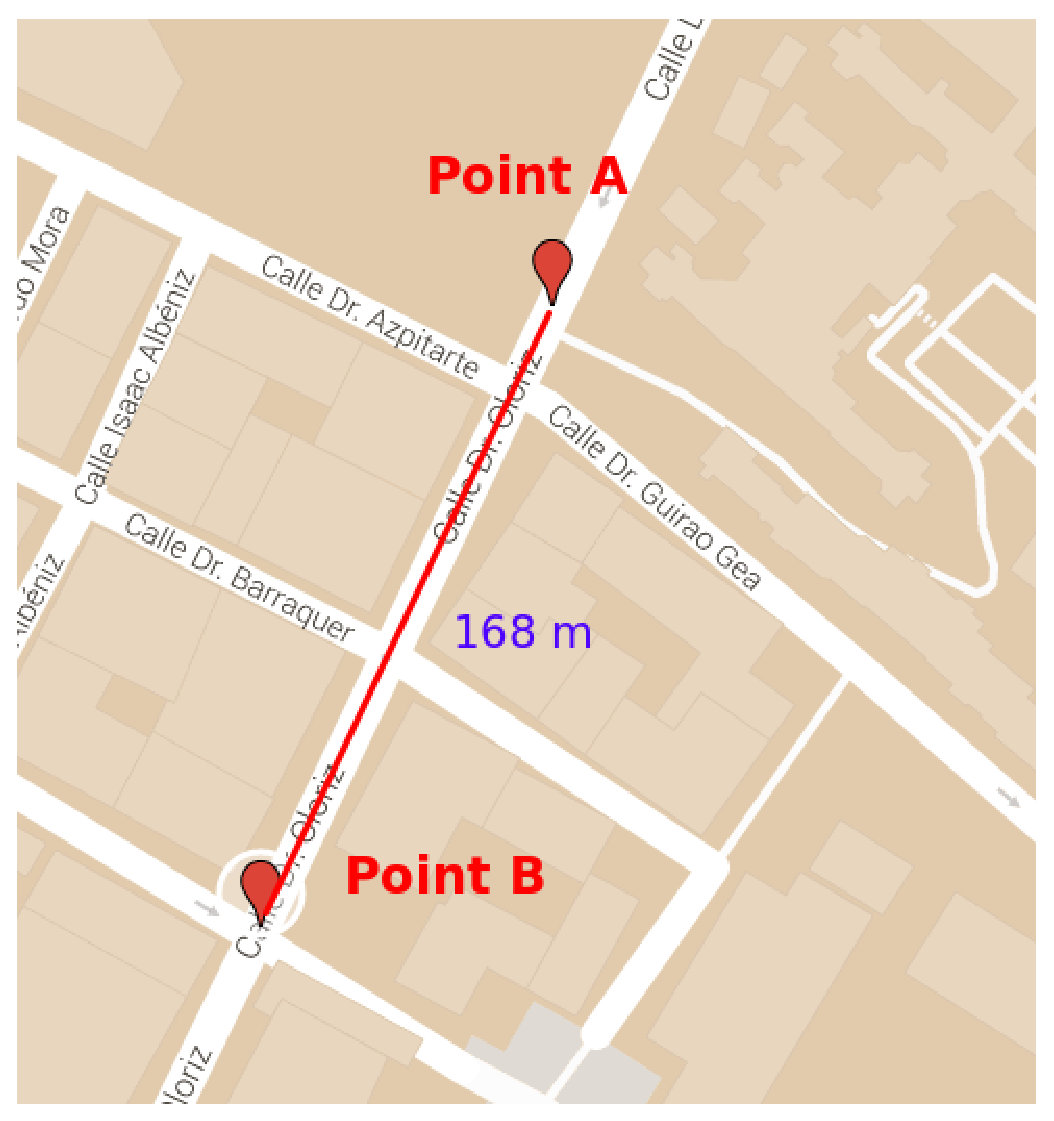
\includegraphics[scale=0.4]{imgs/mososMapa.eps}
		\caption{Urban nodes location in Granada city.}
	\label{fig:mososMapa}
	\end{center}
\end{figure}

\begin{figure}[htb]
	\begin{center}
		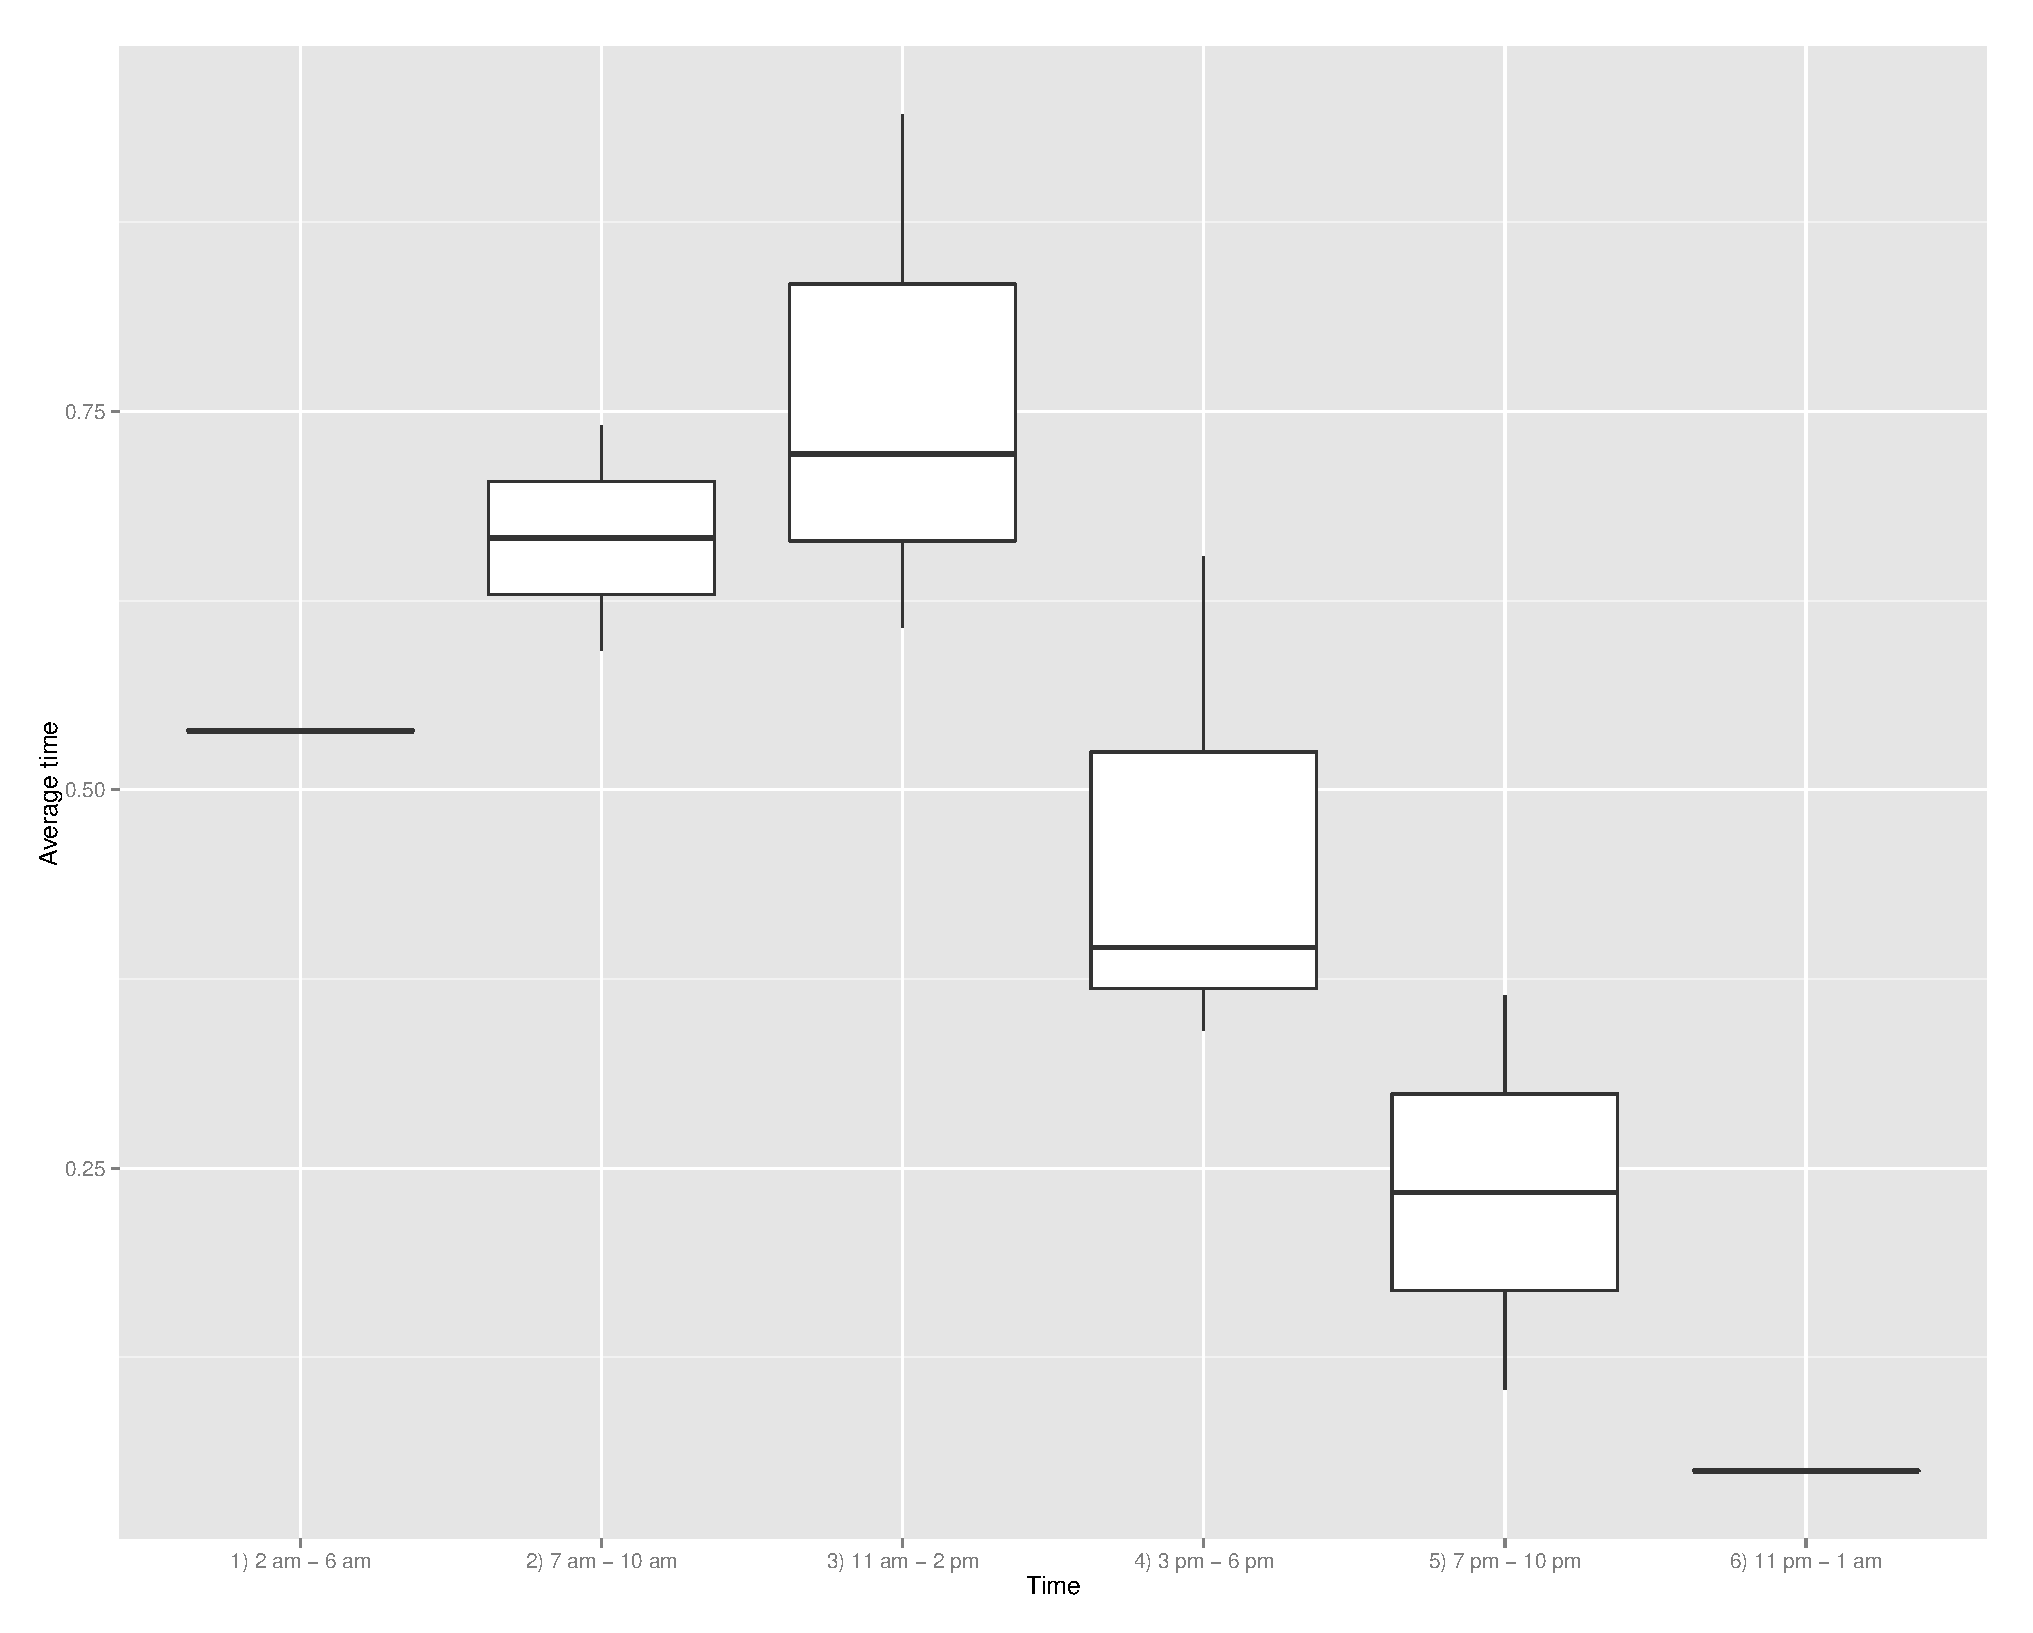
\includegraphics[scale=0.4]{imgs/MOSOS/mosos_graph_tiempos.eps}
		\caption{Average time along the day for movements from node A to node B. We group the hours of a day using eighth terms. The first and the eighth terms include the night, the second one includes the rush hour for morning beginning is included. The third period includes from 9:00am to 11:59am. The fourth term includes the evening until 2:59pm. The fiveth includes from 3:00pm to 5:59pm, the sixth from 6:00 pm to 9:00pm and the seventh from 9:00pm to 11:59pm. In the boxplot se can see the percentage of increment (up to $0.50$) or decrement (low to $0.50$) of the average time needed to go from A to B along the day.}
	\label{fig:mososTiempo}
	\end{center}
\end{figure}

In short, we demonstrate that only using Mobywit, without any additional data it is easy to know if the trip times are increasing or decreasing along the day. The utility that any council is able to give to this information could be rich and diverse. For example, if any council wants to monitor the streets and links the Mobywit output to the traffic light network, the traffic light regulation could be autonomous depending on the time that a monitored device spends to go from one checkpoint to another. 

%----------------------------------------------------------------------------
%%%%%%%%%%%%%%%%%%%%%%%%%%%%%%%   CONCLUSIONS  %%%%%%%%%%%%%%%%%%%%%%%%%%%%%%%
%----------------------------------------------------------------------------

\section{Conclusions}
\label{sec:conclusions}

In this work, MOBYWIT, a novel monitoring and tracking system which gathers mobility data from people and vehicles has been presented. Some of its applications have been shown, using the data collected by the system to address different issues in a city in order to do it `smarter'.
Thus, four different scenarios have been studied:

\begin{itemize}
    \item A discotheque, which has been used as a `stress test' for the system and also to address issues on marketing, energetic efficiency and security in the building, considering the mobility of people inside it on different nights. Clustering methods have been applied in order to visualise and extract interesting knowledge about people's movements and recurrences to the disco.
    \item A public building of the University of Granada, in which students', teachers' and other staff's movements have been analysed using origin/destination matrices with a similar objective than before: security, access improvements and (possibly) marketing reasons.
    \item An interurban road, where the traffic flows have been studied and contrasted with real traffic data, using statistical methods. Moreover forecast techniques have been applied with very good results in the short-term.
% Antonio - VICTOR, revisa que esto sea verdad. ;)
    \item An urban street, which is one of the main arteries of the city of Granada, so it is usually collapsed. A statistical analysis has been conducted to study the traffic flows, detecting possible jams. This information could be potentially used in order to improve the light signal synchronisations in that street.
\end{itemize}

The aim of the work was to show that the results of these studies could be the basis for solving the commented issues, as well as to prove the value and reliability of the presented system. Which has been demonstrated.

Since this paper is a kind of `proof of concept' for MOBYWIT, several future lines of research are open.
Firstly, a deeper study on every issue addressed in the work can be done, focusing on every scenario, considering bigger amounts of data and applying some other techniques, which would improve the quality of the results. Moreover, we could aim to improve the methods of the state of the art for different problems, such as traffic forecast, for instance, but considering our gathered real data.

Also, some other problems in the city could be addressed using MOBYWIT devices, for instance, analysing people's and traffic mobility in the city, in order to improve services (to the tourists, for instance), conduct geo-marketing analyses \cite{Flyers-GeoMarketing,LaMarca-GeoMarketing}, increase the security mechanisms, or improve the public transport system.
This would require the deployment of several devices around the city, in order to better build mobility graphs, origin/destination matrices and other mobility models.

The system itself has some flaws or weak points that could be improved, such as avoiding the overlapping between detections in two different nodes (using unidirectional antennas or some kind of filters or blocking panels).

Another point of improvement could be the use of Time Series Forecast techniques in order to complete `holes' in the detected `events' when there is a power cutoff on a device.

%%%%%%%%%%%%%%%%%%%%%%%%%%%%%  ACKNOWLEDGEMENTS %%%%%%%%%%%%%%%%%%%%%%%%%%%%%%%%

\section*{Acknowledgements}

This work has been supported in part by projects EPHEMECH (TIN2014-56494-C4-3-P, Spanish Ministry of Economy and Competitivity), PETRA (SPIP2014-01437, funded by Dirección General de Tráfico), PYR-2014-17 (GENIL project, awarded by CEI-BIOTIC Granada), and MOSOS (This work has been supported by the project with reference PRY142/14, which has been granted by Fundación Pública Andaluza Centro de Estudios Andaluces in the call 'IX Convocatoria de Proyectos de Investigación). We also thank the DGT and local council of Granada city, and their staff and researchers for their dedication and professionalism. 
%FERGU: le meto un poco la pelota a los de la DGT, con vuestro permiso :)


% ---------------------- BIBLIOGRAFÍA -----------------------

\bibliographystyle{elsarticle-num}
\bibliography{mobility}


% ------------------------- APÉNDICE -----------------------


\section{Appendix} 

This appendix presents additional information about the scenarios, such as the geographical position of the nodes and a comment about them, or some graphs showing the distribution of the gathered data.

\subsection*{Discotheque}

\subsection*{Building of the University}

\begin{table}
\centering
\resizebox{12cm}{!}{
\begin{tabular}{|c|c|p{5cm}|c|c|}
\hline
ID   &  Location & Latitude & Longitude \\ \hline
42	 &  ETSIIT Parking & 37.197377 & -3.6247944\\ \hline
52	 &  ETSIIT Main access of Students& 37.196729 &  -3.62435722\\ \hline
62	 &  ETSIIT Main access of Staff & 37.196928 & -3.6244201\\ \hline
\end{tabular}
}
\caption{Location of the devices for the Building of the University scenario.}
\label{tab:nodosETSIIT}
\end{table}


\subsection*{Highway}

\begin{table}
\centering
\resizebox{12cm}{!}{
\begin{tabular}{|c|c|p{5cm}|c|c|}
\hline
ID   & Province & Location & Latitude & Longitude \\ \hline
1010 & Granada  & A-44 K.P. 118+300 increasing direction (link A-44 K.P. 118+300 with A-92 K.P. 241+000) & 37.241668  & -3.6526 \\ \hline
1020 & Granada  & A-92 K.P. 294+300 increasing direction  & 37.318763 & -3.137978 \\ \hline
1030 & Granada  & A-92 K.P. 344+950, increasing direction & 37.141298 & -2.710871 \\ \hline
1040 & M{\'a}laga  & A-7  K.P. 241+800, decreasing direction (Link A-7 K.P. 241+800 with A-45 K.P. 142+400) &  36.757427 & -4.426879 \\ \hline
1050 & M{\'a}laga  & A-45 K.P. 121+700, decreasing direction & 36.910454 & -4.444769 \\ \hline
1060 & Granada & A-92 K.P. 177+900, decreasing direction (Link A-92 with A-92M) & 37.136209 & -4.282619 \\ \hline
\end{tabular}
}
\caption{Location of the devices for the highway traffic scenario (K.P. = Kilometric Point).}
\label{tab:nodosHighway}
\end{table}


\subsection*{Traffic in a city}

\begin{table}
\centering
\resizebox{12cm}{!}{
\begin{tabular}{|c|c|p{5cm}|c|c|}
\hline
A	 & Granada & Dr. Olóriz Street & 37.188187 & -3.607241\\ \hline
B	 & Granada & Dr. Olóriz Street & 37.186997 & -3.607882\\ \hline
\end{tabular}
}
\caption{Location of the devices for the highway traffic scenario (K.P. = Kilometric Point).}
\label{tab:nodosDGT}
\end{table}



\end{document}
